%--------------------------------------------------
% INSTRUÇÕES / INSTRUCTIONS / INSTRUCCIONES 
%--------------------------------------------------

% Este arquivo é o template oficial da RBIE para artigos redigidos em PORTUGUÊS.

% For English: use main-en.tex
% Para español: use main-es.tex

% Não troque a opção de idioma em \documentclass.

%----- MOTOR DE COMPILAÇÃO
% Recomendado: XeLaTeX ou LuaLaTeX
% NÃO adicione \usepackage[utf8]{inputenc}: UTF-8 já é nativo no LaTeX moderno e o pacote é obsoleto neste template.

%----- O QUE EDITAR NESTE PREÂMBULO
% 1. \title / \engtitle / \thirdlangtitle -- títulos nos três idiomas
% 2. \author{} -- nomes, ORCIDs e e-mails

%----- REFERÊNCIAS
% 1. O padrão bibliográfico APA 7ª edição já está definido no estilo 'apalike-sol.bst'; NÃO ALTERE.
% 2. Insira as entradas bibliográficas no arquivo refs.bib 

%-----  PACOTES JÁ CARREGADOS PELA CLASSE (não redeclare):
    % algorithm, algpseudocode
    % amsmath, amssymb
    % babel
    % caption
    % cuted
    % enumitem
    % etoolbox
    % fancyhdr
    % fontawesome
    % geometry
    % graphicx
    % hyperref
    % listings
    % microtype
    % minted
    % natbib
    % tcolorbox
    % titlesec
    % xcolor
%--------------------------------------------------



% ---- ACESSIBILIDADE: geracao de PDF marcado (tagged PDF / PDF/UA) ----
% Esta linha DEVE permanecer antes de \documentclass. Ela ativa a marcacao estrutural automatica exigida pelas Diretrizes de Acessibilidade para o Conteúdo da Web (WCAG) e pelas orientacoes de acessibilidade da Comissão para Inclusão, Diversidade e Equidade (CIDE) da Sociedade Brasileira de Computação (SBC): cabecalhos, listas, tabelas e ordem de leitura expostos a leitores de tela. Define ainda o idioma do PDF (/Lang) e o padrao PDF/UA-2 (ISO 14289-2), norma internacional de acessibilidade universal para arquivos PDF.
% Requer TeX Live 2024 ou posterior (o Overleaf atual atende). Em TeX Live 2023 ou anterior as chaves 'tagging'/'pdfstandard' nao existem, e a compilacao falha: nesse caso, atualize a distribuicao. Valide o PDF final (ver Secao de figuras).
\DocumentMetadata{
  lang          = pt-BR,
  pdfversion    = 2.0,
  pdfstandard   = ua-2,
  tagging       = off
}

\documentclass[portuguese]{rbie2026}%

% Controla o comportamento e a posição das notas de rodapé
\usepackage[bottom]{footmisc}

%% O pacote tabularray é o mais moderno e abrangente disponível para construção de tabelas. Ele substitui os pacotes tabularx, multirow, multicol, colortbl, longtable
% https://ctan.org/pkg/tabularray
\usepackage{tabularray}

% Ativa os comandos do pacote clássico 'booktabs': \toprule, \midrule, \bottomrule e \cmidrule dentro do ambiente tblr:
\UseTblrLibrary{booktabs}

% Formata números e unidades conforme o Sistema Internacional de Unidades (SI)
\usepackage{siunitx}

%% Highlight code and demos with l3regex and LPeg
% Ativa comando \fakeverb{}, mais robusto que o comando nativo \verb||
\usepackage{codehigh}

% Formata endereços web em fonte monoespaçada
\usepackage{url}

% Evita linhas viúvas e órfãs
% Prevent widow/club lines
\clubpenalty  = 100000000
\widowpenalty = 100000000


%----- HEADER INFORMATION. DO NOT EDIT -----------
%----- RESERVED FOR EDITORS ONLY
\jid{RBIE}
\jtitle{Revista Brasileira de Informática na Educação, 20XX, VV:1}
\issn{1414-5685 (print), 2317-6121 (online)}
\doi{10.5753/rbie.yyyy.id}
\copyrightstatement{This work is licensed under a Creative Commons Attribution 4.0 International License}
\jyear{20XX}

\category{Artigo de Pesquisa / Research Paper / Artículo de investigación}
    
    % --- Alternativas:
    % \category{Artigo estendido / Extended Paper / Artículo extendido}
    
    % \category{Edição Especial / Special Issue / Edición especial}

% initial page number
% \setcounter{page}{889}
%--------------------------------------------------



%----- ACESSIBILIDADE: metadados do PDF -----
% Preencha com o titulo e as pessoas autoras em TEXTO SIMPLES (sem comandos LaTeX, sem cores, sem "--"). O leitor de tela anuncia o \pdftitle no lugar do nome do arquivo (ja habilitado por pdfdisplaydoctitle=true na classe).
\hypersetup{pdftitle={Apresentação do template da RBIE para 2026: versão para artigos em português},
            pdfauthor={Alexandre Direne; José Valente; Liane Tarouco}
            }


%----- PAPER TITLE -------------------------------

% Title in Portuguese [Short title]{Long title}
\title[Título curto do artigo em português]{Apresentação do template da RBIE para 2026 -- Versão para artigos em português}

% Title in English [long title only]
\engtitle{\textcolor{engtitle}{Presenting the RBIE template for 2026 -- Version for works in Portuguese}}

% Title in Spanish [long title only]
\thirdlangtitle{\textcolor{thirdlangtitle}{Presentación de la plantilla RBIE para 2026 -- Versión para artículos en portugués}}
%--------------------------------------------------


%----- AUTHOR INFORMATION ------------------------
%----- THE ORCID IS MANDATORY FOR EACH AUTHOR IN RBIE
      
%----- SUBMISSÃO ANÔNIMA
% Para avaliação anônima:
% 1. Comente todo o bloco \author{}
% 2. No corpo do texto, substitua nomes e afiliações por texto neutro
% 3. Leia Seção 3.3.1 para mais detalhes

\author[
    % Short author/year
    Direne 20XX (1 autor) | Direne \& Tarouco 20XX (2 autores) | Direne et al. 20XX (3 ou mais autores)
    ]{
    
    % Author 1 info
        \affil{\textbf{Alexandre Ibrahim Direne} \thinspace \orcidlink{0000-0000-0000-0000} \thinspace \textcolor{blue}{\faEnvelopeO} \enspace [{Universidade Federal do Paraná} \thinspace | \thinspace \href{mailto:alexd@inf.ufpr.br}{{\textit{alexd@inf.ufpr.br}}}]}
    
    % Author 2 info
        \affil{\textbf{José Armando Valente} \thinspace \orcidlink{0000-0002-1347-186X} \enspace [{Universidade Estadual de Campinas} \thinspace | \thinspace \href{mailto:jvalente@unicamp.br}{{\textit{jvalente@unicamp.br}}}]}
    
    % Author 3 info
        \affil{\textbf{Liane Margarida Rockenbach Tarouco} \thinspace \orcidlink{0000-0002-5669-588X} \enspace [{Universidade Federal do Rio Grande do Sul} \thinspace | \thinspace \href{mailto:liane@penta.ufrgs.br}{{\textit{liane@penta.ufrgs.br}}}]}
}
%--------------------------------------------------


\begin{document}

%----- Elementos pré-textuais (front matter)

\begin{frontmatter}
    \maketitle

    % Corresponding mail address
    \begin{mail}
        Departamento de Informática, Centro Politécnico, Universidade Federal do Paraná, R. Evaristo F. Ferreira da Costa, 383--391, Jardim das Américas, Curitiba, PR, 81530-090, Brasil.
    \end{mail}

%----- Abstract and keywords in the three languages
    % Abstract in Portuguese
    \begin{abstract-pt}
        \textit{Introdução.} Processos editoriais em revistas científicas demandam aprimoramento contínuo para acompanhar a evolução das práticas de pesquisa e das exigências de transparência e reprodutibilidade. \textit{Métodos.} Este artigo apresenta o novo modelo de artigo da Revista Brasileira de Informática na Educação (RBIE), descrevendo sua estrutura e suas recomendações metodológicas para os mais diversos tipos de pesquisa em Informática na Educação. O modelo foi desenvolvido somente no formato \LaTeX\, contemplando três línguas. \textit{Resultados.} O modelo consolida em um único documento convenções dispersas em exemplos anteriores, reduzindo inconsistências de formatação e simplificando a avaliação por pares. \textit{Discussão.} A adoção deste modelo contribui para a padronização editorial da RBIE e para a melhoria da qualidade metodológica dos artigos submetidos. O resumo em português deve vir antes do resumo em inglês (\emph{abstract}), seguido pelo resumo em espanhol (\emph{resumen}). O resumo deve conter entre 150 e 300 palavras.
    \end{abstract-pt}

    % Keywords in Portuguese
    \begin{pchaves}
        Revista Brasileira de Informática na Educação; Template de artigo; Escrita científica. [Informe de 3 a 10 palavras-chave que favoreçam a indexação e a recuperação do artigo nas principais bases de busca de publicações científicas. Use ponto-e-vírgula como separador. As palavras-chave devem iniciar com letra maiúscula.]
    \end{pchaves}

    % Abstract in English
    \begin{abstract-en}
        \textit{Introduction.} Editorial processes in scientific journals require continuous improvement to keep pace with the evolution of research practices and the growing demands for transparency and reproducibility. \textit{Methods.} This article presents the new article template of the Brazilian Journal of Computers in Education -- \emph{Revista Brasileira de Informática na Educação} (RBIE), describing its structure and its methodological recommendations for the most diverse types of research in Computers in Education. The template was developed only in the \LaTeX\ format, covering three languages. \textit{Results.} The template consolidates into a single document conventions that were previously scattered across earlier examples, reducing formatting inconsistencies and simplifying peer review. \textit{Discussion.} The adoption of this template contributes to RBIE's editorial standardization and to the improvement of the methodological quality of submitted articles. For papers written primarily in English, only the abstract in English is required. The abstract should contain between 150 and 300 words.
    \end{abstract-en}

    % Keywords in English
    \begin{keywords}
        Brazilian Journal of Computers in Education; Article template; Scientific writing. [Provide 3 to 10 keywords that facilitate the indexing and retrieval of the article in the main scientific publication databases. Please use semicolons as separators. Keywords must begin with capital letters.]
    \end{keywords}

    % Abstract in Spanish
    \begin{abstract-es}
        \textit{Introducción.} Los procesos editoriales en las revistas científicas requieren un perfeccionamiento continuo para acompañar la evolución de las prácticas de investigación y las exigencias de transparencia y reproducibilidad. \textit{Métodos.} Este artículo presenta el nuevo modelo de artículo de la Revista Brasileña de Informática en la Educación -- \emph{Revista Brasileira de Informática na Educação} (RBIE), describiendo su estructura y sus recomendaciones metodológicas para los más diversos tipos de investigación en Informática en la Educación. El modelo fue desarrollado únicamente en el formato \LaTeX\, contemplando tres idiomas. \textit{Resultados.} El modelo consolida en un único documento convenciones que antes estaban dispersas en ejemplos anteriores, reduciendo inconsistencias de formato y simplificando la evaluación por pares. \textit{Discusión.} La adopción de este modelo contribuye a la estandarización editorial de la RBIE y a la mejora de la calidad metodológica de los artículos enviados. El resumen en portugués debe aparecer antes del resumen en inglés (\emph{abstract}), seguido por el resumen en español. El resumen debe contener entre 150 y 300 palabras.
    \end{abstract-es}

    % Keywords in Spanish
    \begin{pclaves}
        Revista Brasileña de Informática en la Educación; Plantilla de artículo; Redacción científica. [Indique de 3 a 10 palabras clave que favorezcan la indexación y recuperación del artículo en las principales bases de búsqueda de publicaciones científicas. Utilice punto y coma como separador. Las palabras clave deben comenzar con mayúscula.]
    \end{pclaves}

% EDITION DATES. DO NOT EDIT. RESERVED FOR EDITORS ONLY
    \begin{dates}
        {\sffamily\textbf{Received:}} DD Month YYYY \enspace\textbullet\enspace
        {\sffamily\textbf{Accepted:}} DD Month YYYY \enspace\textbullet\enspace
        {\sffamily\textbf{Published:}} DD Month YYYY
    \end{dates}

\end{frontmatter}

%----- Fim dos elementos pré-textuais



%------ Início do texto do manuscrito
\section{Introdução ao modelo de artigo da RBIE}
\label{sec:intro}

Solicitamos que as pessoas autoras interessadas em submeter seus trabalhos de pesquisa à Revista Brasileira de Informática na Educação (RBIE) sigam as orientações deste modelo, a fim de garantir uma apresentação padronizada. Leia atentamente este guia, pois ele apresenta informações importantes sobre ética, orientações metodológicas e instruções sobre formatação. Os manuscritos que não estiverem em formato adequado poderão ser rejeitados pelos editores a qualquer momento no processo de revisão e publicação.

Os nomes das pessoas autoras listados neste template são uma homenagem póstuma a três pesquisadores que dedicaram suas carreiras ao desenvolvimento da Informática na Educação no Brasil, não tendo nenhum deles participado de sua elaboração.

\subsection{Escopo da RBIE}

A RBIE tem por objetivo disseminar ferramentas, métodos e práticas que auxiliam no uso efetivo da tecnologia no processo educativo. Embora o foco inicial da RBIE fosse exclusivamente em trabalhos de pesquisa na área de Informática na Educação, hoje também acolhe e publica trabalhos de pesquisa na área de Educação em Computação.

Apesar de guardarem algumas características comuns, é importante estabelecer as diferenças entre as áreas de Informática na Educação e Educação em Computação. Conforme apontam \cite{Bispo2020}, a pesquisa em Informática na Educação se refere ao uso de artefatos tecnológicos como mediadores nos processos de ensino e aprendizagem, bem como aos seus impactos. Já a Educação em Computação tem como objetivo principal o aperfeiçoamento dos processos de ensino e aprendizagem da Computação como ciência \citep{holmboe2001research}.


\subsection{Recomendações para redigir a seção de Introdução}

A seção de ``Introdução'', ou título equivalente, deve contextualizar o problema de pesquisa, identificar a lacuna que o trabalho pretende preencher e enunciar explicitamente as contribuições do artigo. Recomendamos a seguinte organização típica \citep{ecarnort_writing_article_2015}:

\begin{enumerate}
  \item \textbf{Contextualização (o conhecido).} Apresente o cenário no qual o problema se insere, apoiando-se em evidências da literatura. Evite afirmações genéricas sem respaldo bibliográfico.
 
  \item \textbf{Problema e lacuna (o desconhecido).} Delimite o problema específico investigado e aponte o que a literatura ainda não respondeu plenamente. A lacuna deve ser demonstrada, não apenas declarada.
 
  \item \textbf{Objetivo e questões de pesquisa.} Enuncie o objetivo
  geral do trabalho. Quando aplicável, apresente as questões de pesquisa (QPs) de forma explícita e numerada. Esta é uma prática consolidada em Informática na Educação e facilita a avaliação dos revisores.
 
  \item \textbf{Contribuições.} Liste as principais contribuições do
  trabalho de forma concisa. O uso de marcadores (\texttt{\textbackslash begin\{itemize\}} ou \texttt{\textbackslash begin\{enumerate\}}) é aceitável neste ponto, a critério das pessoas autoras.
 
  \item \textbf{Organização do artigo.} Opcionalmente, descreva em um parágrafo final como as demais seções do manuscrito estão estruturadas.
\end{enumerate}
 
Para artigos de revisão ou mapeamento sistemático, a introdução deve incluir, adicionalmente, a justificativa para a realização de uma revisão secundária sobre o tema, demonstrando que não existe revisão equivalente recente ou que a revisão existente apresenta limitações relevantes.

Essas recomendações de estrutura não são rígidas e podem ser adaptadas às características específicas de cada trabalho de pesquisa.


%------------------------------------------
\section{Instruções Específicas para \LaTeX}
\label{sec:latex}

A classe \texttt{rbie2026} é projetada para trabalhar com os motores (\textit{engines}) \texttt{XeLaTeX} e \texttt{LuaLaTeX}. Dessa forma, deve-se compilar o documento:

\begin{enumerate}
    \item No Overleaf. Acesse \textbf{Menu $>$ Configurações $>$ Compilador} e ajuste a opção ``Compilador'' para \texttt{XeLaTeX} ou \texttt{LuaLaTeX}.\footnote{Os motores-base são denominados \texttt{XeTeX} e \texttt{LuaTeX}. Já a combinação dos motores com as macros \LaTeX formam o \texttt{XeLaTeX} e o \texttt{LuaLaTeX}.}

    \item Na sua instalação local. Configure o editor ou IDE (por exemplo, TeXstudio, TeXworks ou VS~Code) para usar o \texttt{XeLaTeX} ou o \texttt{LuaLaTeX} como compilador. Alternativamente, compile pelo terminal com \texttt{xelatex arquivo} ou \texttt{lualatex arquivo}. Não é necessário informar a extensão \texttt{.tex}.
\end{enumerate}

A classe \texttt{rbie2026} não funciona plenamente com o motor \texttt{pdfLaTeX}. Se você tentar usá-lo para compilar, vai receber mensagens de aviso sobre pacotes de fontes não definidos, e o PDF será gerado com glifos ausentes nos ícones do pacote \texttt{fontawesome}, que depende de fontes Unicode não suportadas pelo motor \texttt{pdfLaTeX}.


\subsection{Diferenças entre \texttt{fontenc} e \texttt{fontspec}}

Os pacotes \texttt{fontenc} e \texttt{fontspec} controlam o gerenciamento de fontes e caracteres no \LaTeX. Eles pertencem a épocas e motores de compilação diferentes: o \texttt{fontenc} é usado no motor clássico (\texttt{pdfLaTeX}), enquanto o \texttt{fontspec} é obrigatório para motores modernos baseados em Unicode (\texttt{XeLaTeX} ou \texttt{LuaLaTeX}).

A distribuição \textbf{TeX Live}, usada pelo Overleaf para preparação de documentos \LaTeX, instala uma vasta gama de fontes: por exemplo, o \textit{TeX Gyre Termes}\footnote{\url{http://www.gust.org.pl/projects/e-foundry/tex-gyre}} é o equivalente livre e gratuito da fonte \textit{Times New Roman}. Para os motores \texttt{XeLaTeX} ou \texttt{LuaLaTeX}, não é obrigatório incluir o pacote \texttt{fontspec}. A omissão faz o motor assumir valores padrões para fonte e suas propriedades\footnote{Por simplicidade o termo \textsc{fonte} está sendo usado como sinônimo do termo \textsc{typeface}. No entanto, os profissionais de tipografia distinguem os dois termos.}.


%------------------------------------------
\section{Organização do Manuscrito}
\label{sec:organization}

O manuscrito deverá conter \textbf{entre 10 e 20 páginas}, excluindo as declarações complementares, as referências e os anexos.


\subsection{Configuração da página}

O tamanho do papel deve ser A4 (210 x 297 mm). As margens do documento devem ter as seguintes medidas:

\begin{itemize}
    \item Superior: 1{,}0 cm
    \item Inferior: 2{,}0 cm
    \item Esquerda: 1{,}8 cm
    \item Direita: 1{,}7 cm
\end{itemize}

Esses valores já estão configurados neste template. Não altere as dimensões das margens, pois qualquer texto fora do padrão poderá atrasar ou até mesmo inviabilizar a publicação do seu artigo na RBIE.


\subsection{Títulos}


\begin{table*}[ht]
    \centering
    \caption{Exemplos de formatação do título.}
    \label{tab:titulo}
    \begin{tblr}{%
        colspec = {ll},
        cells   = {font=\small}
        }
        \toprule
        \textbf{Incorreto} & \textbf{Correto} \\
        \midrule
        APRENDIZAGEM DE PROGRAMAÇÃO COM JUÍZES ONLINE
            & Aprendizagem de Programação com Juízes Online \\
        aprendizagem de programação com juízes online
            & Aprendizagem de Programação com Juízes Online \\
        Aprendizagem De Programação Com Juízes Online
            & Aprendizagem de Programação com Juízes Online \\
        \bottomrule
        \end{tblr}
\end{table*}


As recomendações a seguir sobre a elaboração de títulos se dividem em dois tipos: como escolher as palavras mais adequadas e como formatar a grafia delas.

\subsubsection{Escolha um Título Atraente}

Elabore um título estratégico, descrevendo o escopo, o delineamento e o objetivo do estudo. Recomendamos as seguintes dicas \citep{herbst2024structuring,ecarnort_writing_article_2015}:

\begin{enumerate}
  \item \textbf{Seja conciso e claro.} O título deve ser curto e direto, permitindo que o leitor infira rapidamente o conteúdo da publicação.

  \item \textbf{Evite formulações imprecisas.} Evite termos que não agregam valor informativo, como ``um relato de\ldots'' ou ``um estudo sobre\ldots''. Se os efeitos forem importantes, o título deve declarar quais são exatamente.

  \item \textbf{Identifique o delineamento do estudo.} Tipos específicos de delineamento, como revisões sistemáticas, mapeamentos sistemáticos e experimentos controlados, devem ser explicitamente identificados no título.

  \item \textbf{Destaque o achado principal.} Sempre que possível, o título deve indicar se a intervenção aumenta, reduz ou previne algo.

  \item \textbf{Coloque o aspecto mais importante primeiro.} Se o foco é a intervenção ou a ferramenta investigada, inicie o título com esse elemento para distinguir o artigo de outros sobre o mesmo tema.

  \item \textbf{Use palavras-chave.} O título deve conter os termos principais para que o artigo seja facilmente recuperado em bases de dados como SBC-OpenLib (SOL), ACM Digital Library, IEEE Xplore e Scopus.

  \item \textbf{Desperte o interesse.} O título deve ser suficientemente cativante para incentivar o leitor potencial a acessar o trabalho completo.

  \item \textbf{Diferencie seu trabalho.} O título deve evidenciar como o artigo contribui para a literatura ou preenche uma lacuna no conhecimento da área.

  \item \textbf{Identifique revisões e mapeamentos sistemáticos.} No caso de estudos secundários e terciários, o título deve identificar se o artigo trata de um mapeamento sistemático (ou de uma revisão sistemática), de um estudo terciário, de uma atualização de uma revisão sistemática já existente, ou se inclui uma meta-análise \cite{Kitchenham2023_SEGRESS_supp}.
\end{enumerate}


\subsubsection{Formate o Título} \label{sec:formatacao_titulo}

O título do manuscrito deve seguir estas convenções de formatação:

\begin{enumerate}
  \item \textbf{Formatação tipográfica.} Para o título no idioma original, utilize fonte \textit{Roboto}, tamanho 18pt, alinhado à esquerda, com espaçamento entre linhas de 20pt e estilo em negrito. Se o idioma original do manuscrito for português ou espanhol, os títulos nos idiomas secundários devem utilizar fonte \textit{Roboto}, tamanho 14pt, alinhado à esquerda, espaçamento entre linhas de 12pt, em negrito e itálico, cor cinza (RGB 128, 128, 128).

  \item \textbf{Capitalização (\textit{title case}).} O título deve ser escrito com apenas a inicial de cada palavra em maiúscula. Devem ter inicial \textbf{maiúscula}: a primeira palavra do título (sempre); substantivos, adjetivos, verbos e advérbios; e nomes próprios, incluindo nomes de sistemas, ferramentas e plataformas (ex.: Python, Moodle). Devem permanecer em \textbf{minúsculas} (exceto quando iniciam o título): artigos (o, a, os, as, um, uma); preposições curtas (de, do, da, em, para, por, com, sob, sobre); e conjunções (e, ou, mas, que, se).

  \item \textbf{Caixa alta é vedada.} O título não deve ser digitado inteiramente em letras maiúsculas, mesmo que se deseje dar destaque ao trabalho. A Tabela~\ref{tab:titulo} apresenta exemplos de formatação incorreta e correta de títulos.

  \item \textbf{Evite acrônimos.} O título deve, idealmente, ser livre de siglas para garantir clareza e acessibilidade ao leitor não especialista.

  \item \textbf{Não termine com ponto.} Títulos não fazem parte do texto corrido, por isso não devem terminar com ponto.
\end{enumerate}



\subsection{Informações sobre as Pessoas Autoras}

Para as informações sobre as pessoas autoras (nome, ORCID, afiliação, e-mail), use fonte \textit{Roboto}, tamanho 10pt, alinhamento à esquerda, com espaçamento entre linhas de 8pt e estilo normal, sem espaçamento adicional.

Na fase de submissão do manuscrito, todas as informações que possam identificar a autoria devem ser suprimidas. Caso o trabalho seja aceito, essas informações devem ser preenchidas nos metadados do formulário de submissão, bem como na versão final do texto do manuscrito.


\subsubsection{Anonimização do Manuscrito}

Para garantir a integridade da avaliação duplamente anonimizada, observe estas recomendações para a primeira versão a ser submetida:

\begin{itemize}
    \item \textbf{Pessoas autoras e afiliações.} Omita nomes, afiliações institucionais e endereços de todas as pessoas autoras. Os campos correspondentes no template devem ser preenchidos com \textit{Omitido para revisão}.

    \item \textbf{Agradecimentos.} Suprima a seção de agradecimentos, pois ela frequentemente identifica financiadores, orientadores ou projetos vinculados às pessoas autoras.

    \item \textbf{Financiamento e bolsas.} Não mencione agências de fomento, números de processo ou projetos de pesquisa que possam identificar as pessoas autoras ou suas instituições.

    \item \textbf{Localização dos experimentos.} Não mencione a cidade onde os experimentos ou coletas de dados foram realizados. Mencione o estado ou a região somente se esse dado for relevante para a avaliação de mérito.

    \item \textbf{Plataformas e sistemas institucionais.} Não mencione nomes de plataformas, sistemas, ambientes virtuais de aprendizagem ou ferramentas desenvolvidas pelas próprias pessoas autoras que possam identificá-las. Quando necessário, utilize denominações genéricas, como \textit{o jogo utilizado} ou \textit{a plataforma de submissão adotada}.

    \item \textbf{Links e URLs.} Não inclua hiperlinks que contenham informações identificadoras, como nomes de usuário, nomes de repositórios pessoais ou institucionais, ou domínios de instituições. Repositórios de dados ou materiais suplementares devem ser anonimizados por meio de serviços como o \textit{Anonymous GitHub} (\url{https://anonymous.4open.science/}) antes da submissão.

    \item \textbf{Autocitações.} Ao citar trabalhos próprios, utilize formulações neutras como \textit{[omitido para revisão]} no lugar da referência bibliográfica, evitando frases como \textit{``como demonstramos em [X]''} ou \textit{``em trabalho anterior, nós investigamos...''}.

    \item \textbf{Metadados do arquivo.} Verifique e remova os metadados do arquivo PDF antes do envio, pois eles podem conter o nome do autor, a instituição ou o software utilizado na edição. No Linux, o comando \texttt{exiftool -{}-all= arquivo.pdf} realiza essa limpeza; no Windows e macOS, o mesmo resultado pode ser obtido por meio das propriedades do documento.

    \item \textbf{Figuras e capturas de tela.} Certifique-se de que imagens, diagramas e capturas de tela não exibam logotipos institucionais, nomes de usuário, endereços de e-mail ou quaisquer outros elementos identificadores.

    \item \textbf{Questionários e instrumentos de pesquisa.} Caso o manuscrito descreva instrumentos e questionários aplicados em uma instituição específica, remova (ou generalize) referências ao contexto institucional nos enunciados e exemplos reproduzidos no texto.
\end{itemize}


\subsubsection{Restauração de Autoria após Aceitação do Manuscrito}

Após a aceitação definitiva do manuscrito, submeta a versão final com todas as informações restauradas, incluindo nomes, afiliações, agradecimentos e referências completas. Para cada pessoa autora, as informações deverão ser apresentadas na seguinte sequência:

\begin{enumerate}
    \item Nome completo da pessoa, sem abreviações
    
    \item Link para o perfil ORCID (\textit{Open Researcher and Contributor ID})\footnote{\url{https://orcid.org/}}.
    
    \item Quando for o caso, indicar qual a pessoa autora para correspondência, por meio do símbolo \textcolor{blue}{\faEnvelopeO}.
    
    \item Nome da instituição à qual a pessoa autora está afiliada.
    
    \item Endereço de e-mail.
\end{enumerate}


\subsection{Resumo e Palavras-chave}

O resumo é a seção mais lida de um artigo científico. Provavelmente, será a única lida antes de se decidir pela leitura completa do trabalho. Ele deve oferecer uma visão geral do manuscrito, contemplando seus objetivos, metodologia, principais resultados e conclusões. Aqui seguem algumas recomendações para planejar a estrutura do resumo, refinar sua linguagem e estilo, remover equívocos comuns e formatá-lo.


\subsubsection{Planejamento da Estrutura do Resumo}

Planeje e estruture o conteúdo do resumo antes de desenvolver as frases, conforme as orientações a seguir \citep{ecarnort_writing_article_2015}:

\begin{enumerate}
  \item \textbf{Escreva por último.} Redija o resumo após a conclusão de todas as demais seções do manuscrito, pois somente então é possível sintetizá-lo com precisão.

  \item \textbf{Seja autossuficiente.} O resumo deve funcionar como um documento independente: o leitor deve compreendê-lo integralmente sem precisar consultar o texto completo.

  \item \textbf{Adote o formato IMRAD.} Recomenda-se adotar a estrutura padrão composta por Introdução, Métodos, Resultados e Discussão (\textit{Introduction, Methods, Results And Discussion}) \citep{abstract_Nundy2022}.

  \item \textbf{Responda a quatro perguntas fundamentais:}
  \begin{enumerate}
    \item Por que você começou? (Introdução/Objetivo)
    \item O que você fez? (Métodos)
    \item O que você encontrou? (Resultados)
    \item O que isso significa? (Conclusões/Implicações)
  \end{enumerate}

  \item \textbf{Inclua dados reais.} Nos resultados, evite termos subjetivos (muitos, poucos) e apresente dados quantitativos específicos, como valores \textit{p}, intervalos de confiança, percentuais ou números absolutos.

  \item \textbf{Seja honesto(a) com os resultados.} Relate os desfechos principais mesmo que não sejam estatisticamente significativos; evite discutir apenas ``tendências'' sem sustentação empírica.
\end{enumerate}


\subsubsection{Linguagem e Estilo}

Após elaborar a estrutura do resumo, revise as escolhas linguísticas e estilísticas conforme as sugestões a seguir, para tornar o resumo mais claro e acessível ao leitor:

\begin{enumerate}
  \item \textbf{Use voz ativa.} Prefira construções na voz ativa (ex.: ``Conduzimos um experimento\ldots'') em vez da passiva, pois tornam a leitura mais direta e objetiva.

  \item \textbf{Empregue o tempo verbal adequado.} Use o tempo passado para descrever o que foi feito e o que foi encontrado.

  \item \textbf{Evite jargões.} Não utilize termos técnicos excessivamente complexos nem siglas pouco familiares ao público-alvo. Defina todas as siglas na primeira ocorrência.

  \item \textbf{Prefira frases simples.} Opte por sentenças declarativas curtas e diretas, com uma ideia principal por frase.
\end{enumerate}


\subsubsection{O que Evitar na Redação do Resumo}

Os itens listados a seguir comprometem a qualidade da redação de resumos:

\begin{enumerate}
  \item \textbf{Não inclua citações.} Resumos geralmente não devem conter referências a outros trabalhos publicados. Exceções: atualizações de uma revisão sistemática, continuação ou refutação de um estudo anterior específico.

  \item \textbf{Não recorte frases do corpo do texto.} O resumo deve ser redigido do zero, e não composto por trechos literalmente recortados das demais seções.

  \item \textbf{Garanta a consistência interna.} Verifique se os dados apresentados no resumo são idênticos aos que constam nas tabelas e no corpo do texto.
\end{enumerate}


\subsubsection{Formatação}

Para formatar o resumo e as palavras-chave, adote as orientações a seguir:

\begin{enumerate}
  \item \textbf{Extensão.} O resumo deve conter entre \textbf{150 e 300 palavras}. A última frase deve terminar com ponto final.

  \item \textbf{Tipografia e alinhamento.} O texto do resumo deve ser justificado, com espaçamento entre linhas simples, sem espaçamento antes e depois do parágrafo, em fonte \textit{TeX Gyre Termes}, tamanho 9pt.

  \item \textbf{Palavras-chave.} Na linha seguinte ao resumo, forneça o título ``Palavras-chave:'' em fonte \textit{Roboto}, tamanho 9pt, negrito. Ele deve ser seguido de 3 a 10 palavras-chave, em fonte \textit{TeX Gyre Termes}, tamanho 9pt, alinhadas à esquerda, com espaçamento entre linhas simples, sem espaçamento antes e com espaçamento de 24pt depois. Use o \textbf{ponto-e-vírgula} como separador. As palavras-chave devem ser grafadas com iniciais maiúsculas.

  \item \textbf{Idiomas obrigatórios.} O número de resumos exigidos varia conforme o idioma principal do manuscrito:
  
  \begin{itemize}
    \item Artigos em \textbf{português}: além do resumo em português (nativo), forneça o resumo e as palavras-chave também em inglês (\textit{abstract}) e em espanhol (\textit{resumen}), nesta ordem.
    
    \item Artigos em \textbf{espanhol}: além do resumo em espanhol (nativo), forneça somente a versão em inglês (\textit{abstract}) e as palavras-chave correspondentes.
    
    \item Artigos em \textbf{inglês}: forneça apenas o resumo em inglês (nativo). Não é necessário fornecer resumo nem palavras-chave em português ou em espanhol.
  \end{itemize}
\end{enumerate}



\subsection{As Seções}

O documento deve ser organizado em duas colunas, com o texto justificado em fonte \textit{TeX Gyre Termes}, tamanho 10pt, espaçamento entre linhas simples. O primeiro parágrafo da seção, subseção e sub-subseção não tem recuo na primeira linha; os demais parágrafos têm recuo de 0{,}71\,cm (20pt).

Os títulos seguem as regras de capitalização da Seção~\ref{sec:formatacao_titulo}. As formatações específicas de cada nível são detalhadas a seguir.


\subsubsection{Títulos das Seções}

O título de uma seção deve ser grafado em negrito, fonte \textit{Roboto}, tamanho 14pt, com as letras iniciais maiúsculas, alinhado à esquerda com espaçamento entre linhas simples, com espaçamento adicional de 10pt antes e 4pt depois. Após o número do título, não deve haver ponto.

\subsubsection{Títulos de Subseções}

O título de uma subseção deve ser grafado em negrito, fonte \textit{Roboto}, tamanho 12pt, com as letras iniciais maiúsculas, alinhado à esquerda com espaçamento entre linhas simples, com espaçamento adicional de 8pt antes e 1pt depois. Após o número do título, não deve haver ponto.

\subsubsection{Títulos de Sub-subseções}

O título de uma sub-subseção deve ser grafado em negrito itálico, fonte \textit{Roboto}, tamanho 11pt, com as letras iniciais maiúsculas, alinhado à esquerda com espaçamento entre linhas simples, com espaçamento adicional de 7pt antes e 1pt depois. Após o número do título, não deve haver ponto.



%------------------------------------------
\section{Trabalhos Relacionados}
\label{sec:related-work}

A seção de ``Trabalhos Relacionados'' visa posicionar o trabalho no contexto da literatura existente, fundamentar as escolhas metodológicas e evidenciar a originalidade da contribuição. Recomendamos a seguinte organização:
 
\begin{enumerate}
  \item \textbf{Critérios de seleção da literatura.} Descreva, ainda que brevemente, como os trabalhos relacionados foram identificados (bases de dados consultadas, termos de busca, período coberto). Isso confere transparência ao processo de revisão de literatura, mesmo em artigos de pesquisa primária, em que a revisão da literatura não precisa seguir o rigor de uma revisão sistemática, conforme \cite{Kitchenham2023_SEGRESS}.
 
  \item \textbf{Organização temática.} Agrupe os trabalhos relacionados por tema ou abordagem, não apenas em ordem cronológica. Para cada grupo, sintetize o que foi feito, quais resultados foram obtidos e quais limitações foram reportadas. Evite escrever uma sequência de parágrafos no estilo \textit{O trabalho de X fez Y. O trabalho de Z fez W}, sem análise crítica ou comparativa.
 
  \item \textbf{Diferenciação.} Encerre a seção com um parágrafo (ou subseção) que articule explicitamente como o presente trabalho se diferencia ou complementa os estudos discutidos. Este parágrafo conecta a revisão ao problema enunciado na introdução.
\end{enumerate}

Para artigos de \textbf{revisão sistemática ou mapeamento sistemático}, adicionamos estas recomendações:

\begin{enumerate}
    \item Esta seção de ``Trabalhos Relacionados'' deve ser adaptada para apresentar o referencial teórico (conceitos, modelos e teorias que fundamentam a revisão) ou um levantamento de outros estudos secundários já realizados anteriormente. Já a  literatura encontrada pelos critérios de inclusão e exclusão deve ser analisada na seção de ``Resultados'' (ou equivalente).

    \item Verifique se a base de dados consultada em sua revisão inclui a RBIE e a biblioteca SOL. A ausência desses repositórios na string de busca compromete a cobertura de um corpo relevante da produção científica brasileira em Informática na Educação.
\end{enumerate}



\begin{table*}[ht]
    \centering
    \caption{Comandos de citação do pacote \texttt{natbib} disponíveis no template da RBIE 2026, com exemplos.}
    \label{tab:natbib}
    \begin{tblr}{%
        colspec  = {Q[l,m]
               Q[l,m,0.4\linewidth]
               Q[l,m]},
        cells    = {font=\small}
        }
        \toprule
        \textbf{Comando} & \textbf{Situação} & \textbf{Efeito} \\
        \midrule
        %%%
        \textbf{Citações básicas} & & \\
        \midrule
        %%%
        % \lstinline$\cite{chave}$ & & \\
          \fakeverb{\cite{chave}} &
          Autor integrado na frase; ano entre colchetes &
          conforme \cite{Wohlin2012} \\
        %
          \fakeverb{\citep{chave}} &
          Referência parentética completa ao final da frase &
          \citep{Cohen1988} \\
        %
          \fakeverb{\citep[p.~XX]{chave}} &
          Citação parentética com página ou seção específica &
          \citep[p.~15]{Cohen1988} \\
        %%%
        \midrule
        \textbf{Citações com notas adicionais} & & \\
        \midrule
        %%%
          \fakeverb{\cite[p.~XX]{chave}} &
          Autor na frase; com página ou seção específica &
          \cite[p.~15]{Cohen1988} \\
        %
          \fakeverb{\citep[ver][]{chave}} &
          Citação parentética com prefixo textual &
          \citep[ver][]{Wohlin2012} \\
        %
          \fakeverb{\citep[ver][cap.~Z]{chave}} &
          Citação parentética com prefixo e sufixo &
          \citep[ver][cap.~3]{Wohlin2012} \\
        %
          \fakeverb{\citep[][cap.~Z]{chave}} &
          Citação parentética apenas com sufixo &
          \citep[][cap.~3]{Cohen1988} \\
        %%%
        \midrule
        \textbf{Elementos isolados} & & \\
        \midrule
        %%%
          \fakeverb{\citeauthor{chave}} &
          Apenas o nome do autor, sem ano &
          \citeauthor{Cohen1988} \\
        %
          \fakeverb{\citeyear{chave}} &
          Apenas o ano, sem delimitadores &
          \citeyear{Cohen1988} \\
        %
          \fakeverb{\citeyearpar{chave}} &
          Apenas o ano entre colchetes &
          \citeyearpar{Cohen1988} \\
        %%%
        \midrule
        \textbf{Múltiplas referências} & & \\
        \midrule
        %&&
          \fakeverb{\citep{a,b,c}} &
          Várias referências agrupadas em uma única citação parentética;
          listar preferencialmente em ordem cronológica &
          \citep{Cohen1988,Wohlin2012} \\
        \bottomrule
    \end{tblr}
\end{table*}


\subsection{Citações e Referências Bibliográficas}

A lista de referências deve registrar com precisão e completude todas as fontes citadas no texto, permitindo que o leitor as localize de forma independente. A RBIE adota o estilo \textbf{APA 7ª edição} \citep{APAStyleTeam2020coronavirus} para formatação das referências. As orientações a seguir cobrem as informações mínimas exigidas, as diretrizes gerais do estilo e os formatos específicos por tipo de obra.

\begin{enumerate}
  \item \textbf{Correspondência entre citações e lista.} Toda obra citada no corpo do artigo deve constar na lista de referências, e vice-versa. Referências não citadas não devem integrar a lista.
 
  \item \textbf{Ordenação alfabética.} Liste as referências em ordem alfabética pelo último sobrenome do(a) primeiro(a) autor(a). Em caso de múltiplas obras de mesma autoria (ou  autorias), ordene pelo ano de publicação, do mais antigo para o mais recente.
 
  \item \textbf{Citação no texto.} Siga o formato autor-data do estilo APA~7 para as citações no texto: \textbf{[Sobrenome, Ano]} para citações no interior de colchetes e \textbf{Sobrenome [Ano]} quando o nome do autor integra a frase. Para obras com três ou mais pessoas autoras, utilize o último sobrenome do primeiro autor seguido de ``\textit{et al.}'' já na primeira citação. Por exemplo: Tarouco \textit{et al.} [2015].
 
  \item \textbf{DOI e URL.} Inclua o DOI sempre que disponível, formatado como hiperlink (\texttt{https://doi.org/xxxxx}). Na ausência de DOI, inclua a URL de acesso estável à publicação. Evite URLs de buscadores, encurtadores ou repositórios intermediários quando a fonte primária estiver disponível.
 
  \item \textbf{Idioma da referência.} As referências devem ser registradas no idioma original da obra, sem tradução dos títulos. Quando o título estiver em alfabeto não latino, inclua uma transliteração entre colchetes.
 
  \item \textbf{Consistência interna.} Adote um único critério para abreviação dos nomes das pessoas autoras, capitalização de títulos e pontuação, e mantenha-o em todas as entradas da lista de referências.

   \item \textbf{Informações essenciais.} Toda entrada bibliográfica deve conter estas quatro informações, necessariamente nesta ordem (estilo APA):
   
   \begin{enumerate}
       \item autoria (pessoas ou instituições)
       \item ano de publicação
       \item título da obra
       \item local de publicação (editora, periódico ou evento, URL, instituição etc.)
   \end{enumerate}
\end{enumerate}


\subsubsection{Erros a evitar nas referências}

\begin{enumerate}
  \item \textbf{Referências incompletas.} Não omita campos obrigatórios (volume, número de páginas, DOI), pois isso impede a localização da obra e compromete a credibilidade do seu trabalho.

  \item \textbf{Citação de fontes secundárias.} Evite citar uma obra por meio de outra (``\textit{apud}''). Localize e leia a fonte primária. Quando isso for genuinamente impossível, indique a fonte secundária no texto e registre apenas a fonte secundária na lista de referências, conforme as diretrizes do APA~7~\citep{APAStyleTeam2020coronavirus}.

  \item \textbf{URLs instáveis ou de acesso restrito.} Links para  páginas de busca, sessões autenticadas ou repositórios institucionais de acesso restrito não permitem recuperar a fonte. Prefira DOI e URL permanentes de repositórios abertos.

  \item \textbf{Preprints apresentados como artigos publicados.} Preprints não passaram por revisão por pares e não devem ser referenciados como se fossem artigos publicados em periódico. Se existir uma versão revisada e publicada do mesmo trabalho, cite-a em lugar do preprint.

  \item \textbf{Inconsistência na grafia dos nomes de autores.} O mesmo autor não deve aparecer com grafias diferentes ao longo da lista  de referências (por exemplo, com variação no número de iniciais).

  \item \textbf{Omissão da lista completa de autores.} Na lista de referências, indique o nome de todos os autores de cada obra. Algumas ferramentas automáticas substituem --- erroneamente --- o nome do segundo ao último autor por ``\textit{et al.}'' ou equivalente, destoando do estilo APA~7~\citep{APAStyleTeam2020coronavirus}. Verifique e corrija antes de submeter seu manuscrito.
\end{enumerate}



\subsection{Como Citar Obras no \LaTeX}

A RBIE adota o pacote \texttt{natbib} para gerenciamento de citações, configurado com o estilo \textbf{autor-ano} e delimitadores em \textbf{colchetes}. O pacote disponibiliza um conjunto de comandos que permite você controlar com precisão a forma como cada referência é integrada ao texto. A Tabela~\ref{tab:natbib} apresenta os principais comandos disponíveis, organizados por categoria de uso, com exemplos e o respectivo efeito tipográfico produzido, considerando a configuração adotada neste template. É possível incluir notas adicionais, como números de página ou seções, por meio do argumento opcional dos comandos, conforme exemplificado na tabela.

 

%------------------------------------------
\section{Metodologia}
\label{sec:methods}

A seção de metodologia deve fornecer informações suficientes para que o estudo possa ser avaliado criticamente e, quando pertinente, replicado. A organização varia conforme o tipo de pesquisa.
 
\subsection{Pesquisa Primária} 

Quando o manuscrito relata uma pesquisa primária (experimento, estudo de caso, survey, pesquisa de design), recomendamos abordar os seguintes elementos, divididos em subseções quando necessário:
 
\begin{enumerate}
  \item \textbf{Delineamento da pesquisa.} Identifique e justifique o método adotado, de forma coerente com as questões de pesquisa. A série de livros CEIE/SBC\footnote{\url{https://ceie.sbc.org.br/metodologia/}}~\citep{mpcie_vol1_concepcao_pesquisa, mpcie_vol2_pesquisa_quanti, mpcie_vol3_pesquisa_quali} apresenta os principais métodos usados na área, entre os quais: experimento controlado e quase-experimento~\citep{mpcie_vol2_cap2_experimentos}, estudo de caso~\citep{mpcie_vol3_cap1_estudo_caso}, survey, \textit{Design Science Research}~\citep{mpcie_vol1_cap5_design_science_research}, pesquisa-ação~\citep{mpcie_vol3_cap2_pesquisa_acao} e estudo longitudinal. Consulte \citep{mpcie_vol1_cap4_tipos_pesquisa} para uma visão geral das classificações de pesquisa adotadas na área.
 
  \item \textbf{Participantes.} Descreva o perfil dos participantes (número, nível de formação, instituição, período no curso), o processo de recrutamento e os procedimentos éticos adotados, incluindo aprovação em comitê de ética, quando o experimento envolver intervenções realizadas diretamente com seres humanos \citep{mpcie_vol1_cap7_etica}.
 
  \item \textbf{Instrumentos e materiais.} Descreva os instrumentos utilizados para coleta de dados (questionários, ferramentas computacionais, rubricas de avaliação), indicando, quando aplicável, sua validade e confiabilidade previamente reportadas na literatura. Conforme \cite{Bittencourt_Isotani_2018_Evidencias}, instrumentos previamente validados pela literatura são preferíveis a instrumentos de avaliação desenvolvidos sem rigor metodológico. Para o desenvolvimento e validação de questionários na área de Informática na Educação, consulte \cite{mpcie_vol2_cap6_questionarios}.

  \item \textbf{Procedimentos.} Descreva a sequência de atividades realizadas, incluindo o cronograma, as condições de aplicação e qualquer controle experimental adotado.
 
  \item \textbf{Análise dos dados.} Descreva os métodos de análise empregados, indicando as referências metodológicas adotadas \citep{creswell2023research}. Para \textbf{abordagens quantitativas}, informe os testes estatísticos e critérios de significância adotados; consulte \cite{mpcie_vol2_cap9_descritiva} e \cite{mpcie_vol2_cap10_inferencial} para orientações específicas. Para \textbf{abordagens qualitativas}, especifique a técnica de análise adotada, pois cada uma tem pressupostos epistemológicos distintos e não são intercambiáveis (por exemplo, análise de conteúdo~\citep{mpcie_vol3_cap9_analise_conteudo}, análise do discurso~\citep{mpcie_vol3_cap7_analise_discurso}, análise hermenêutica~\citep{mpcie_vol3_cap8_analise_hermeneutica}, entre outras). Informe também a medida de confiabilidade entre avaliadores, quando aplicável (por exemplo, Kappa de Cohen~\citep{Cohen1960}).
\end{enumerate}


\subsection{Revisão Sistemática ou Mapeamento Sistemático} 

O protocolo de seleção de estudos deve ser descrito de forma estruturada, cobrindo os seguintes elementos~\citep{Kitchenham2023_SEGRESS_supp, mpcie_vol2_cap3_rsl}:
 
\begin{enumerate}
  \item \textbf{Questões de pesquisa (QPs).} Apresente as QPs que orientam a revisão, preferencialmente estruturadas com base em um framework adequado (por exemplo, PICO, PICOC ou equivalente). Para orientações específicas ao contexto de Informática na Educação, consulte \citep{mpcie_vol2_cap3_rsl}.
 
  \item \textbf{String de busca e bases de dados.} Apresente a string de busca utilizada e as bases de dados consultadas, justificando as escolhas. Informe o período coberto e a data de execução da busca.
 
  \item \textbf{Critérios de inclusão e exclusão.} Liste os critérios de forma explícita. Critérios ambíguos comprometem a reprodutibilidade do estudo.
 
  \item \textbf{Processo de seleção.} Descreva as etapas de triagem (leitura de título e resumo, leitura completa) e informe o número de estudos em cada etapa. O uso de um diagrama de fluxo de seleção é fortemente recomendado.
 
  \item \textbf{Extração e síntese dos dados.} Descreva o formulário de extração de dados e o processo de síntese adotado. Para revisões com dois ou mais pesquisadores, informe a medida de concordância inter-avaliadores utilizada (por exemplo, Kappa de Cohen~\citep{Cohen1960}).
 
  \item \textbf{Avaliação da qualidade.} Quando aplicável, descreva os critérios de avaliação da qualidade dos estudos primários incluídos.
\end{enumerate}

Antes de submeter o manuscrito, aplique o \textit{checklist} do SEGRESS~\citep{Kitchenham2023_SEGRESS_supp} (\textit{Software Engineering Guidelines for REporting Secondary Studies}) para verificar se todos os elementos obrigatórios da revisão ou mapeamento estão presentes.

%------------------------------------------
\section{Análise e Discussão dos Resultados}
\label{sec:analysis}
 
Esta seção deve apresentar os resultados obtidos e a discussão desses resultados à luz das questões de pesquisa e da literatura. As pessoas autoras podem optar por separar Resultados e Discussão em seções distintas, desde que a organização seja coerente com a natureza do estudo.
 
\begin{enumerate}
  \item \textbf{Organização por questão de pesquisa.} Recomenda-se estruturar a apresentação dos resultados de acordo com as QPs enunciadas na metodologia. Cada QP deve ser respondida com evidências explícitas (dados quantitativos, excertos qualitativos, categorias emergentes).
 
  \item \textbf{Apresentação dos dados.} Utilize tabelas e figuras para sintetizar dados complexos, sempre os referenciando no texto antes de sua apresentação. Tabelas e figuras devem ser autoexplicativas por meio de seus títulos e legendas. 
  
  \item \textbf{Análise dos dados contidos na tabela.} Não narre a tabela em forma de texto corrido, meramente repetindo o conteúdo que já está apresentado em formato tabular. Interprete o significado dos valores e argumente sobre as implicações.
 
  \item \textbf{Relato estatístico.} Para resultados quantitativos, reporte medidas de tendência central e dispersão, o teste estatístico empregado, o valor de~\textit{p} e, obrigatoriamente, o tamanho de efeito (por exemplo, \textit{d} de Cohen, \(\eta^2\) ou equivalente). Resultados estatisticamente significativos, sem relato de tamanho de efeito, são insuficientes para avaliação da relevância prática dos achados.
 
  \item \textbf{Interpretação e discussão.} Contextualize os resultados em relação à literatura revisada. Indique em que medida os achados corroboram, contradizem ou ampliam estudos anteriores. Evite que a discussão se limite a parafrasear os dados já apresentados.
 
  \item \textbf{Revisões sistemáticas.} Para revisões e mapeamentos, organize os resultados em torno das QPs, apresentando sínteses analíticas (não apenas listas de estudos). Utilize recursos visuais como gráficos de distribuição por ano, tema, método ou veículo de publicação quando contribuírem para a compreensão do panorama da área.
\end{enumerate}

As subseções a seguir apresentam recomendações metodológicas e de formatação para elementos não textuais presentes não apenas na seção de ``Análise e Discussão dos Resultados'', mas em qualquer outra do manuscrito.


\subsection{Elementos Não Textuais}

Elementos não textuais são componentes do artigo que comunicam informação por meio de recursos visuais ou estruturais. Exemplos mais comuns: tabelas, figuras, equações, listagens de código e algoritmos.

Três regras se aplicam a qualquer elemento não textual:

\begin{enumerate}
    \item \textbf{Todo elemento deve ser discutido no texto.} O elemento não textual dá suporte à argumentação; ele não fala por si mesmo. Se o texto não precisa discuti-lo para sustentar uma afirmação, o elemento é desnecessário e deve ser removido.

    \item \textbf{A referência precede o elemento.} O texto deve mencionar o elemento antes de ele aparecer na página.

    \item \textbf{A referência é grafada com inicial maiúscula.} Exemplos: Tabela~1, Figura~2, Listagem~3, Algoritmo~4, Caixa~5. Equações são o único caso em que o número é grafado entre parênteses: Equação~(6).
\end{enumerate}

Em todos os elementos não textuais (tabelas, figuras, listagens, algoritmos e caixas), o \textbf{texto da legenda} deve ser formatado assim: fonte \textit{TeX Gyre Termes}, tamanho 8pt, alinhamento justificado, com espaçamento entre linhas simples, espaçamento antes do parágrafo de 6pt, nenhum espaçamento depois. O \textbf{nome do elemento} e a numeração correspondente segue a mesma formatação, mas devem ser destacados em negrito. Use um ponto após a numeração do elemento.

\paragraph{Quadros.} Algumas convenções editoriais brasileiras, em especial a ABNT, distinguem \textbf{tabela} (dados quantitativos, bordas laterais abertas) de \textbf{quadro} (dados qualitativos ou mistos, bordas fechadas). Este template trata ambos como tabelas, mas respeita a distinção quando as pessoas autoras a adotarem de forma consistente no manuscrito.

\paragraph{Como comentar um elemento não textual.} Referências isoladas, tais como ``ver Tabela~1'', ``segundo Figura~2'', ``conforme Listagem~3'', não são uma discussão científica. Com base em \citet{Moskovitz2023}, recomendamos que o trecho do texto corrido que comenta cada elemento não textual execute os seguintes movimentos retóricos. A combinação e a ordem deles variam conforme a seção do artigo.

\begin{enumerate}
  \item \textbf{Anunciar.} Indique ao leitor quando consultar o elemento, referenciando-o pelo nome e número antes de ele aparecer na página. Este é o único movimento obrigatório em todas as seções do artigo.

  \item \textbf{Orientar.} Descreva brevemente o que o elemento representa, especialmente quando o tipo de visualização não é imediatamente óbvio para o público-alvo. Decida o que vai no texto corrido e o que vai na legenda: informações que preparam as pessoas leitoras \textit{antes} de elas olharem para o elemento pertencem ao texto; informações que devem ser consultadas repetidamente \textit{enquanto} analisa o elemento pertencem à legenda.

  \item \textbf{Observar.} Direcione o olhar das pessoas leitoras para as características, tendências ou valores mais relevantes. Observações podem ser pontuais: no caso de tabelas e figuras, um valor específico, pico, \textit{outlier} ou tendência; no caso de listagens e algoritmos, uma operação de especial interesse.

  \item \textbf{Explicar.} Interprete o significado das observações. Responda à pergunta: por que esse padrão ocorre e o que ele implica para o argumento do artigo? Observações sem explicação são uma discussão incompleta.
\end{enumerate}


\subsection{Tabelas}

Tabelas organizam visualmente dados que dão suporte à argumentação. Uma tabela bem construída permite que a pessoa leitora extraia informações e compare valores sem precisar recorrer ao texto. 

As recomendações a seguir tratam de três tópicos sobre construção de tabelas: formatação, aspectos metodológicos e erros a evitar.

\begin{table}[bth]
    \caption{Exemplo de legenda de tabela que ocupa a largura de uma coluna. Legendas de tabelas devem ser posicionadas acima. Fonte dos dados: [indicar].}
    \label{tab:tabela1coluna}
    \centering
    \begin{tblr}{%
        colspec = {cr},
        cells   = {font=\small}
        }
        \toprule
        \textbf{Dimensão} & \textbf{Medida (unidade)}\\
        \midrule
         1  &  1,6232 \\
         2  &  2,9635 \\ 
         3  &  3,9724 \\ 
         4  &  4,9690 \\ 
         5  &  5,9840 \\ 
         6  &  6,9842 \\ 
         7  &  7,9873 \\ 
         8  &  8,9884 \\
         9  &  9,9873 \\ 
         10 & 10,9898 \\ 
         11 & 11,9914 \\
        \bottomrule
    \end{tblr}
\end{table}


\begin{table*}
    \caption{Exemplo de legenda de tabela que ocupa a largura das duas colunas da página. Legendas de tabelas devem ser posicionadas acima delas. Esta legenda é maior para ocupar o espaço de mais de uma linha.}
    \label{tab:tabela2colunas}
    \centering
    \vspace{-8pt}
    \begin{longtblr}[%
        label=none,
        note{a} = {\footnotesize{Primeira nota de rodapé.}},
        note{$\dag$} = {\footnotesize{Esta é uma segunda nota de rodapé desta tabela, bem mais longa que a primeira, para servir de exemplo mais completo para as mais variadas situações que as pessoas autoras possam necessitar.}},
        remark{\footnotesize{Nota}} = {\footnotesize{Alguma nota geral sobre a tabela.}},
        remark{\footnotesize{Fonte}} = {\footnotesize{Dados inventados pelos criadores do modelo da REIC e reaproveitados no modelo da RBIE.}},
    ]{%
        colspec = {c c c c c c c c c c},
        cells   = {font=\small},
        width = 0.9\linewidth
    }
        \toprule
        \textbf{Número} & \textbf{Vel. (km/h)} &
        $\boldsymbol{\alpha}$ \textbf{(m/s}$\boldsymbol{^2}$\textbf{)} &
        $\boldsymbol{\beta}$ & $\boldsymbol{\gamma}$\TblrNote{a} &
        $\boldsymbol{\delta}$\TblrNote{$\dag$} &
        $\boldsymbol{\epsilon}$ & $\boldsymbol{\zeta}$ &
        $\boldsymbol{\eta}$     & $\boldsymbol{\theta}$ \\*
        \midrule
             1 & 3,5 & 2,0 & 0,20 & $-$0,05 & 0,00 & $-$0,20 & $-$0,05 & 0,20 & 10 \\*
             2 & 2,5 & 1,5 & 0,10 & $-$0,15 & 0,05 & $-$0,15 & ~0,00 & 0,10 & 40 \\*
             3 & 3,0 & 1,8 & 0,20 & $-$0,05 & 0,25 & ~0,05 & ~0,20 & 0,15 & 70 \\*
            \bottomrule
    \end{longtblr}
\end{table*}


\subsubsection{Formatação de Tabelas}
 
\begin{enumerate}
    \item O modelo da RBIE recomenda fortemente o uso do pacote \texttt{tabularray}\footnote{\url{https://ctan.org/pkg/tabularray}} para construção de tabelas. Ele agrega e aprimora as funcionalidades de vários pacotes especializados e bem conhecidos: \texttt{tabularx}, \texttt{multirow}, \texttt{multicol}, \texttt{colortbl}, \texttt{longtable}, \texttt{threeparttablex}.

    \item O tamanho do texto no interior da tabela deve ser menor que no corpo do texto (opção \fakeverb{cells = {font=\small}}) no ambiente \texttt{tblr}.
    
    \item Tabelas podem ocupar uma coluna do texto, como a Tabela~\ref{tab:tabela1coluna}, ou se estender pelas duas colunas, como a Tabela~\ref{tab:tabela2colunas}.
    
    \item Nas tabelas, as legendas devem ser posicionadas \textbf{acima}.
    
    \item Para artigos escritos em português, use a \textbf{vírgula} como separador de casas decimais.
    
    \item Tabelas não devem ter traços verticais. As linhas horizontais devem se limitar apenas ao cabeçalho, rodapé e divisões de seções em tabelas maiores. Tais recomendações visam proporcionar um visual enxuto, com foco nos dados, em vez de linhas.

    \item O alinhamento das colunas numéricas deve refletir a natureza dos valores que elas contêm. Os valores escalares, que exprimem magnitudes, devem ser alinhados à direita (opção \texttt{r}), pois esse alinhamento posiciona os dígitos pela casa decimal e facilita a comparação visual de magnitude. Já os valores ordinais, que apenas identificam ou rotulam as linhas, podem ser alinhadas conforme o estilo das pessoas autoras, uma vez que não representam quantidades a serem comparadas entre si. A Tabela~\ref{tab:tabela1coluna} ilustra essa distinção: a coluna de valores ordinais, à esquerda, é centralizada, ao passo que a coluna de valores escalares, à direita, é alinhada à direita.
\end{enumerate}

\subsubsection{Recomendações Metodológicas}
 
\begin{enumerate}
  \item \textbf{Autonomia informacional.} A legenda e as notas de rodapé da tabela devem ser suficientes para que ela seja compreendida de forma independente do texto corrido. Abreviações, unidades de medida e símbolos utilizados nas células devem ser explicados nas notas ou na legenda.
  
  \item \textbf{Precisão e consistência numérica.} Os valores apresentados devem ser consistentes com os reportados no texto e nos demais elementos do artigo. O número de casas decimais deve ser uniforme dentro de cada coluna e compatível com a precisão do instrumento de medida utilizado. Evite reportar mais casas decimais do que a precisão do método permite \citep{Cole_too_many_digits}. Para amostras menores que 100 indivíduos, apresente percentagens sem casas decimais, por exemplo: 9\% (7/79). Para amostras de 100 ou mais indivíduos, uma casa decimal é adequada, por exemplo: 2{,}8\% (16/580). Em ambos os casos, incluir o numerador e o denominador entre parênteses pode tornar seu texto mais claro a quem lê.
 
  \item \textbf{Unidades de medida.} Informe a unidade de medida de cada coluna ou linha quantitativa, preferencialmente no cabeçalho, e não em cada célula individualmente. Utilize as convenções do Sistema Internacional de Unidades (SI) para representar as medidas, seus símbolos, múltiplos e submúltiplos \citep{Inmetro2025SI}. Recomendamos fortemente o uso do pacote \texttt{siunitx}\footnote{\url{https://ctan.org/pkg/siunitx}} para formatar valores, unidades e derivações conforme as normas do SI.
 
  \item \textbf{Completude dos dados estatísticos.} Ao reportar resultados de testes estatísticos, a tabela deve incluir, quando aplicável, o valor da estatística do teste, o valor de~\textit{p} e o tamanho de efeito. A omissão de qualquer desses elementos compromete a interpretabilidade e a reprodutibilidade dos resultados \citep{Cohen1988}.
 
  \item \textbf{Identificação de valores ausentes.} Células em branco são ambíguas: o dado não existe ou foi esquecido? Por isso, células sem dados devem ser marcadas de forma explícita e consistente, por exemplo com a abreviação ``N/A'' (não aplicável), acompanhadas de nota explicativa. Essa recomendação metodológica atende também às diretrizes de acessibilidade: células vazias prejudicam a leitura da tabela por leitores de tela, e um marcador textual explícito torna a ausência do dado inequívoca para toda pessoa leitora. Não recomendamos o uso de um travessão (---) porque o leitor de tela pode anunciá-lo de forma inconsistente ou simplesmente ignorá-lo.
 
  \item \textbf{Ordenação significativa.} As linhas e colunas devem ser ordenadas de acordo com um critério relevante para a análise (por exemplo, ordem decrescente de frequência, ordem cronológica ou agrupamento por categoria).

  \item \textbf{Declaração da origem dos dados e da ferramenta de geração.} O título, a legenda ou as notas de rodapé da tabela devem identificar a origem dos dados apresentados (coleta própria, base de dados pública, extração de literatura, etc.) e, quando aplicável, a ferramenta utilizada para sua geração ou processamento (por exemplo, planilha eletrônica, linguagem de programação com biblioteca específica, ou sistema de gerenciamento de banco de dados). Quando uma ferramenta de IA generativa for utilizada para produzir, completar ou reorganizar os dados da tabela, isso deve ser declarado explicitamente na ``Declaração de utilização de inteligência artificial (IA)'', localizada no final do artigo, conforme exigido pelo Código de Conduta para autores da SBC \citeyearpar{SBC2024conduta_pt}. Dados gerados por IA sem validação empírica independente não devem ser apresentados como dados primários de pesquisa.
\end{enumerate}

 
\subsubsection{Erros a Evitar em Tabelas}

\begin{enumerate}
  \item \textbf{Redundância com o texto.} Não construa tabelas que apenas repetem dados já apresentados no corpo do texto. Tabelas justificam-se quando os dados são numerosos, multidimensionais ou requerem comparação sistemática.
 
  \item \textbf{Excesso de colunas ou linhas.} Tabelas excessivamente largas dificultam a leitura e frequentemente indicam que os dados poderiam ser reorganizados ou divididos em mais de uma tabela temática.
 
  \item \textbf{Mistura de unidades sem distinção.} Apresentar valores de naturezas distintas (por exemplo, percentuais e valores absolutos) na mesma coluna induz a erros de interpretação, se não houver uma distinção clara.
 
  \item \textbf{Títulos vagos ou excessivamente longos.} A legenda deve identificar com precisão o conteúdo da tabela. Títulos como ``Resultados'' ou ``Dados coletados'' não são informativos.
 
  \item \textbf{Ausência de fonte para dados secundários.} Quando a tabela apresenta dados extraídos de outras fontes, a referência deve ser indicada explicitamente, seja no título, seja em nota de rodapé.
\end{enumerate}
 

\subsection{Figuras}

Pelo termo ``figura'', entendem-se gráficos, diagramas, fluxogramas, capturas de tela, fotografias e qualquer outro elemento visual que comunique dados ou processos. A escolha e a construção de uma figura devem ser orientadas pela pergunta: \textit{o que este elemento visual comunica, mas que o texto ou uma tabela não comunicaria com a mesma eficiência?} 

As recomendações a seguir tratam de três aspectos sobre construção de figuras: formatação, aspectos metodológicos e erros a evitar. Por fim,  são apresentadas considerações éticas e legais sobre imagens que retratam participantes de pesquisa, inclusive crianças.

\subsubsection{Formatação de Figuras}
 
\begin{enumerate}
    \item Figuras podem ocupar apenas uma coluna do texto, como a Figura~\ref{fig:figura1coluna}, ou se estender pelas duas colunas, como a Figura~\ref{fig:figura2colunas}.
    
    \item Nas figuras, as legendas devem ser posicionadas \textbf{abaixo}.

    \item Sempre que possível, as figuras devem ser submetidas em formato vetorial (PDF, SVG ou EPS), e não em formato \textit{raster} (PNG, JPEG, TIFF), também  conhecido como matricial ou baseado em pixels. Formatos vetoriais são independentes de resolução: a figura permanece nítida em qualquer tamanho de exibição, sem serrilhamento. Gráficos gerados por ferramentas como R, Python (\texttt{matplotlib}, \texttt{seaborn}), SPSS ou Inkscape podem ser exportados diretamente em PDF ou SVG. Fotografias e capturas de tela, por sua natureza intrínseca, são exceções aceitas em formato \textit{raster}, desde que com resolução mínima de 300 dpi.

    \item \textbf{Texto alternativo (obrigatório).} Toda figura deve incluir uma descrição textual por meio da chave \texttt{alt} no comando \fakeverb{\includegraphics}, como demonstrado nas Figuras~\ref{fig:figura1coluna} e~\ref{fig:figura2colunas}. Esse texto não aparece no PDF impresso, mas é lido por leitores de tela, atendendo às Diretrizes de Acessibilidade para o Conteúdo da Web (WCAG) \citep{W3C2023wcag22}, cujo uso é recomendado pela Comissão para Inclusão, Diversidade e Equidade (CIDE) da Sociedade Brasileira de Computação (SBC) \citep{sbc2025panorama}. A descrição deve informar o propósito da figura, o tipo de visualização, os eixos e a tendência ou conclusão principal, além de transcrever qualquer texto embutido nela. Comece a descrição pelo próprio conteúdo da figura, pois os leitores de tela já sinalizam que se trata de uma imagem. Por isso, evite dizer ``imagem de'' ou ``foto de''.
\end{enumerate}

\begin{figure}
    \centering
    % ACESSIBILIDADE: a chave 'alt' fornece o TEXTO ALTERNATIVO lido por leitores de tela (exigido pelas Diretrizes de Acessibilidade para o Conteúdo da Web - WCAG). Este texto NAO aparece no PDF impresso. Descreva proposito, tipo de grafico, eixos e a tendencia/conclusao principal. Descreva diretamente o conteudo da figura, sem "imagem de". Sem interpretacoes subjetivas.
    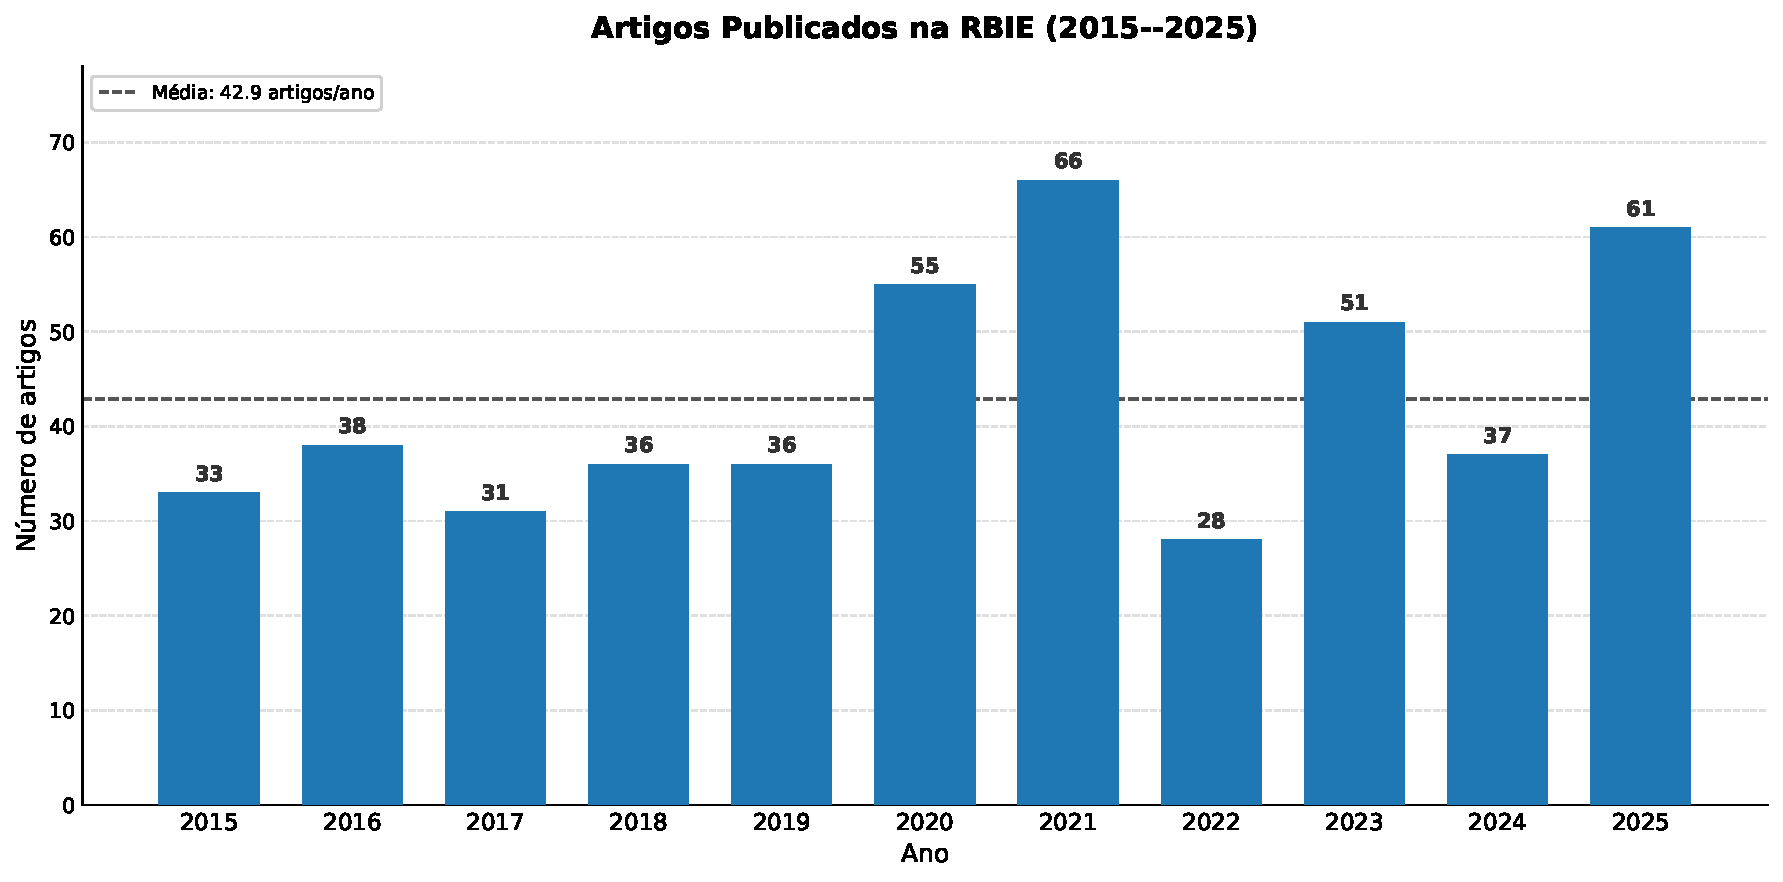
\includegraphics[width=\columnwidth,
      alt={Gráfico de linhas do número de artigos publicados na RBIE por ano. O eixo horizontal indica os anos e o eixo vertical, a quantidade de artigos. A série apresenta tendência geral de crescimento ao longo do período. Substitua esta descrição pela da sua figura.}]{img/rbie_artigos_por_ano.pdf}

    % Legenda da figura, exibida no PDF impresso:
    \caption{Exemplo de legenda de figura. Legendas de figuras devem ser posicionadas abaixo. Gráfico gerado com a biblioteca Matplotlib em Python. Fonte dos dados: RBIE.}
    \label{fig:figura1coluna}
\end{figure}


\begin{figure*}
    \centering
    % ACESSIBILIDADE: veja a nota sobre a chave 'alt' na Figura de uma coluna acima.
    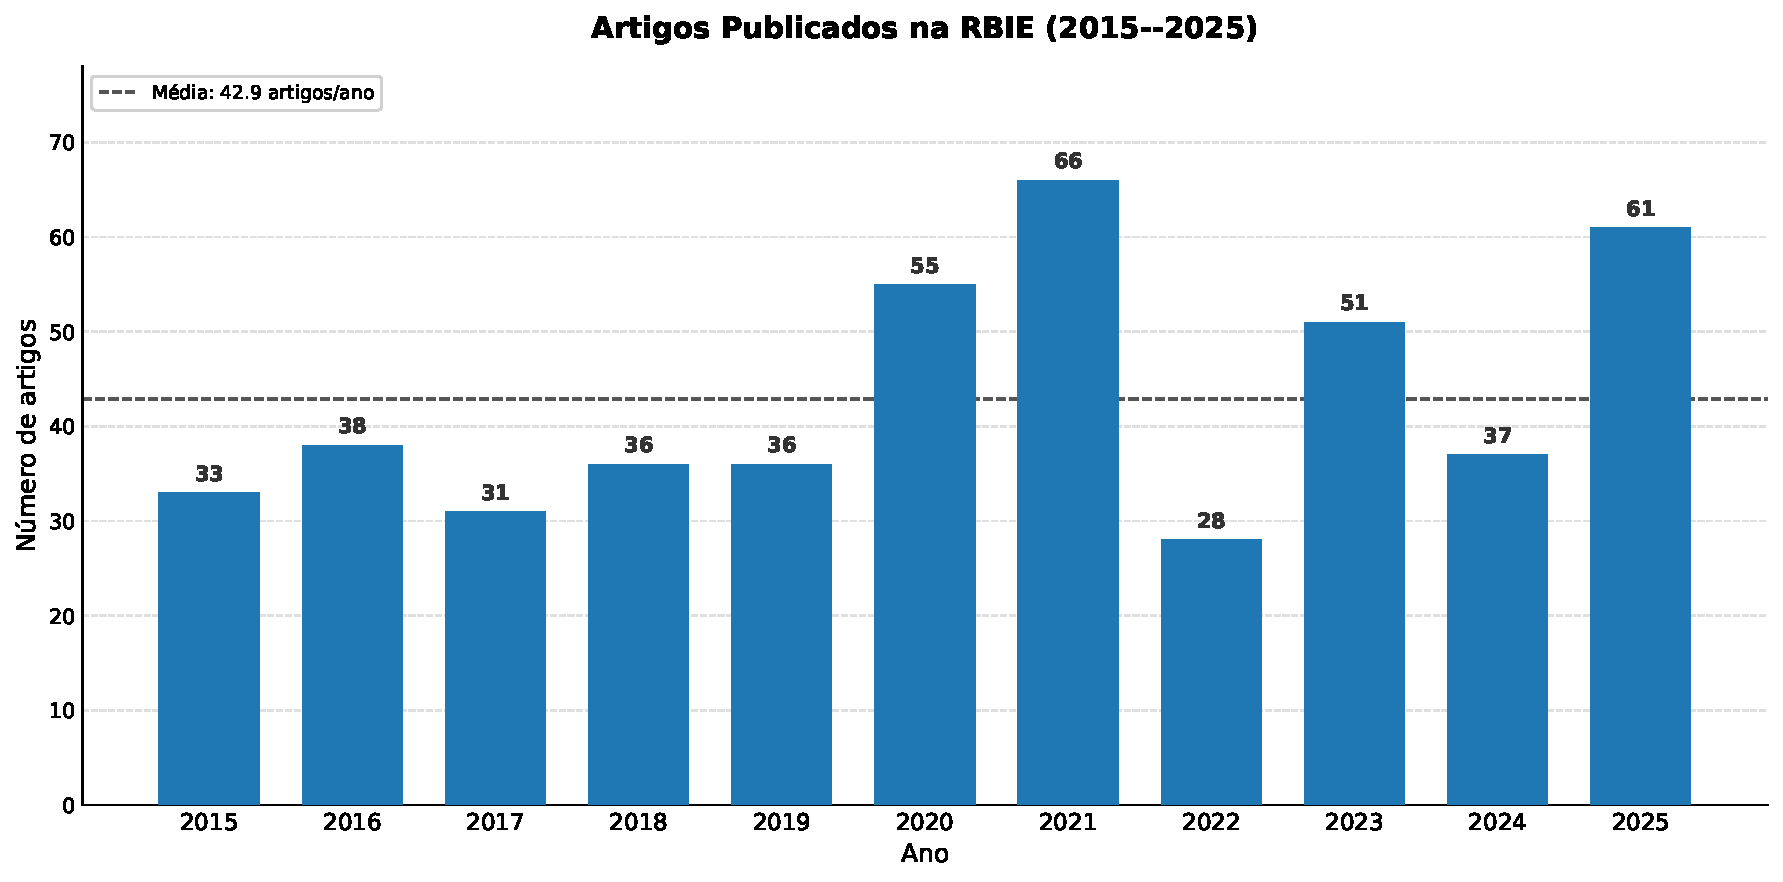
\includegraphics[width=.9\linewidth,
      alt={Gráfico de linhas do número de artigos publicados na RBIE por ano. O eixo horizontal indica os anos e o eixo vertical, a quantidade de artigos. A série apresenta tendência geral de crescimento ao longo do período. Substitua esta descrição pela da sua figura.}]{img/rbie_artigos_por_ano.pdf}
    \caption{Exemplo de legenda de figura. Legendas de figuras devem ser posicionadas abaixo. Gráfico gerado com a biblioteca Matplotlib em Python. Fonte dos dados: RBIE.}
    \label{fig:figura2colunas}
\end{figure*}


\subsubsection{Recomendações Metodológicas}
 
\begin{enumerate}
  \item \textbf{Adequação do tipo de figura ao dado.} O tipo de visualização deve ser coerente com a natureza dos dados, caso contrário distorcerá a interpretação dos dados. Por exemplo, gráficos de barras são adequados para comparar categorias discretas; gráficos de linhas, para exibir tendências ao longo de uma variável contínua ou temporal; diagramas de dispersão, para relacionar duas variáveis quantitativas.
 
  \item \textbf{Autonomia informacional.} A legenda posicionada abaixo da figura deve ser suficiente para que ela seja compreendida independentemente do texto. Eixos, séries, símbolos e cores utilizadas devem ser identificados na própria figura ou na legenda.
 
  \item \textbf{Integridade da representação visual.} A escala dos eixos deve começar em zero quando se trata de grandezas absolutas, salvo justificativa explícita. Escalas truncadas ou não lineares sem aviso explícito distorcem a percepção das diferenças entre valores e constituem erro metodológico.
 
  \item \textbf{Identificação da fonte para dados secundários.} Figuras baseadas em dados de outras fontes devem indicar a referência explicitamente na legenda. Figuras reproduzidas ou adaptadas de outros trabalhos devem indicar a fonte e, quando aplicável, a permissão de uso.
 
  \item \textbf{Diagramas de processo e fluxo.} Fluxogramas, diagramas de sequência e mapas conceituais devem ter notação consistente ao longo de todo o artigo.

   \item \textbf{Origem dos dados e da ferramenta de geração.} A legenda ou o texto do manuscrito deve identificar: (A) a fonte de onde foram extraídos os dados apresentados na figura; e (B) o software ou a ferramenta utilizada para gerar a figura (por exemplo, biblioteca específica do R ou Python). Quando uma ferramenta de IA generativa for utilizada para criar, modificar ou aprimorar a figura, isso deve ser declarado explicitamente na ``Declaração de utilização de inteligência artificial (IA)'', localizada no final do artigo, conforme exigido pelo Código de Conduta para autores da SBC \citeyearpar{SBC2024conduta_pt}. Figuras geradas integralmente por IA sem intervenção metodológica das pessoas autoras (por exemplo, diagramas ou infográficos produzidos por prompt) devem ser evitadas em artigos de pesquisa primária, pois não constituem representação verificável de dados empíricos. Quando utilizadas para fins ilustrativos, devem ser identificadas como tal.
 
  \item \textbf{Figuras de revisão sistemática.} Em artigos de revisão sistemática ou mapeamento, o diagrama de fluxo de seleção de estudos é um elemento obrigatório. Ele deve registrar o número de estudos em cada etapa do processo de triagem, permitindo às pessoas leitoras verificarem a transparência do processo de seleção de estudos.
\end{enumerate}


\subsubsection{Erros a Evitar em Figuras}
 
\begin{enumerate}
  \item \textbf{Figuras decorativas ou redundantes.} Evite incluir figuras cujo conteúdo já está integralmente coberto por uma tabela ou pelo texto. Cada figura deve acrescentar informação ou perspectiva que os demais elementos não oferecem.
 
  \item \textbf{Excesso de variáveis em uma única figura.} Figuras com muitas séries, cores ou dimensões simultâneas dificultam a extração de conclusões. Prefira dividir visualizações complexas em figuras menores e mais focadas.
 
  \item \textbf{Gráficos de pizza para quatro ou mais categorias.} Gráficos de pizza dificultam a comparação precisa entre fatias de tamanho e cores similares. Para quatro ou mais categorias, gráficos de barras oferecem maior precisão perceptual e devem ser preferidos.
 
  \item \textbf{Ausência de barras de erro em dados experimentais.} Gráficos que apresentam médias de dados experimentais sem indicar medidas de dispersão (desvio padrão, erro padrão ou intervalo de confiança) ocultam a variabilidade dos resultados.
 
  \item \textbf{Legendas vagas.} Legendas como ``Resultados do experimento'' não identificam o conteúdo da figura. A legenda deve descrever de forma autocontida o que está sendo exibido, sem que os leitores recorram diretamente ao texto para extrair contexto.
 
  \item \textbf{Capturas de tela como substituto de dados.} Capturas de tela de ferramentas são aceitáveis apenas quando o objetivo é ilustrar a interface em si. Dados numéricos extraídos de ferramentas devem ser apresentados em tabelas ou gráficos construídos pelas pessoas autoras, não como imagens da saída do software.

  \item \textbf{Efeitos tridimensionais em gráficos.} Não aplique efeitos 3D (perspectiva, profundidade, sombra ou extrusão) em gráficos de barras, pizza, linhas ou dispersão. Eles distorcem visualmente as proporções entre os valores, dificultam a leitura das grandezas representadas e não acrescentam informação ao gráfico. A tridimensionalidade é justificada apenas quando os dados têm efetivamente três dimensões analíticas a representar.
\end{enumerate}


\subsubsection{Recomendações sobre Fotografias de Pessoas}

A publicação de fotografias de participantes de pesquisa é regulada pelas seguintes normas de proteção e privacidade:

\begin{itemize}
  
  \item \textbf{No Brasil:}
  
  \begin{itemize}
    \item Lei Geral de Proteção de Dados Pessoais (LGPD) \citep{LGPD2018};
    
    \item Estatuto da Criança e do Adolescente (ECA) \citep{ECA1990};
    
    \item Lei n.º 14.874/2024 \citep{brasil2024lei14874}, regulamentada pelo Decreto n.º 12.651/2025 \citep{brasil2025decreto12651}, que dispõe sobre a pesquisa com seres humanos e institui o Sistema Nacional de Ética em Pesquisa com Seres Humanos, marco legal em vigor desde 2024;

    \item Resoluções CNS n.º 466/2012 \citep{cns2012resolucao466} e n.º 510/2016 \citep{cns2016resolucao510}, que permanecem válidas como referência ética no que não conflitarem com o novo marco legal, durante o período de transição. A Resolução n.º 510/2016 trata especificamente das pesquisas em Ciências Humanas e Sociais, campo em que a maioria dos estudos de Informática na Educação se enquadra; a Resolução n.º 466/2012 é o marco geral e aplica-se de forma subsidiária.
  \end{itemize}
  
  \item \textbf{Internacionalmente:}
  
  \begin{itemize}
    \item Regulamento Geral de Proteção de Dados da União Europeia (GDPR) \citep{GDPR2016};

    \item Diretrizes éticas da \textit{American Psychological Association} (APA).
  \end{itemize}

\end{itemize}


Uma fotografia de um participante de pesquisa não é apenas um elemento decorativo no manuscrito. É um dado pessoal sensível com implicações éticas, legais e humanas. Antes de incluir qualquer imagem que retrate seres humanos, responda mentalmente às seguintes perguntas:

\begin{enumerate}
  \item Esta imagem é cientificamente necessária?
  
  \item Tenho autorização documentada para publicá-la?
  
  \item A publicação preserva a dignidade de quem aparece nela?
\end{enumerate}

As recomendações a seguir orientam esse processo.

\begin{enumerate}
  \item \textbf{Necessidade científica da imagem.} A inclusão de fotografias de pessoas deve ser justificada pela contribuição científica da imagem ao argumento do artigo. Exemplo: fotografias de participantes em situação de interação com ferramentas ou ambientes de aprendizagem são pertinentes quando o contexto espacial ou comportamental for relevante para a análise. Fotografias de confraternização da equipe ou meramente ilustrativas não devem ser incluídas.
 
  \item \textbf{Consentimento livre, esclarecido e documentado.} A publicação de fotografias que permitam a identificação de adultos exige termo de consentimento livre e esclarecido (TCLE) específico para uso da imagem, distinto do TCLE geral da pesquisa. O documento assinado deve ser retido pelos pesquisadores e estar disponível para verificação por parte da equipe editorial da RBIE.
 
  \item \textbf{Autorização dos responsáveis legais para fotografias de crianças.} Para imagens de menores de 18 anos, o consentimento deve ser obtido dos pais ou responsáveis legais, em conformidade com o ECA (artigo 17). Recomenda-se adicionalmente o assentimento da própria criança, quando sua maturidade o permitir, conforme a Resolução CNS n.º 466/2012 \citep{cns2012resolucao466}.
 
  \item \textbf{Anonimização quando o consentimento não for obtido.} Quando não for possível obter consentimento, ou quando a exposição da identidade não for necessária ao argumento científico, a fotografia deve ser anonimizada antes da submissão. Técnicas aceitáveis incluem desfoque ou oclusão da região do rosto e de outros elementos identificadores (tatuagens, uniformes com nome, crachás). A anonimização deve ser aplicada a todas as pessoas identificáveis na imagem, não apenas ao participante focal.
 
  \item \textbf{Declaração no artigo.} As pessoas autoras devem declarar, na seção de ``Declarações Complementares'' ou na seção de ``Metodologia'', que os consentimentos para uso de imagem foram obtidos e que o estudo foi submetido e aprovado pelo Comitê de Ética em Pesquisa (CEP) competente. \textbf{Essa declaração é obrigatória para publicação do estudo na RBIE.} Como o sistema nacional de ética em pesquisa está em reorganização, recomenda-se seguir as orientações vigentes do CEP da instituição das pessoas autoras quanto ao fluxo de submissão e à instância responsável.
  
  \item \textbf{Atenção a contextos de vulnerabilidade.} Fotografias que retratem participantes em situação de vulnerabilidade (estudantes com dificuldades de aprendizagem, populações indígenas, crianças em situação de risco) exigem cuidado redobrado. Nesses casos, mesmo havendo consentimento, as pessoas autoras devem avaliar se a publicação da imagem preserva a dignidade dos participantes e não os expõe a riscos adicionais decorrentes da circulação do artigo.
\end{enumerate}


%------------------------------------------
\subsection{Equações}

Para inserir equações no texto, recomendamos que as pessoas autoras atentem para as seguintes orientações:

\begin{enumerate}
  \item \textbf{Numeração.} Numere todas as equações que sejam referenciadas no texto. Se apenas uma única equação for usada no texto, então a numeração pode ser dispensada. Use o ambiente \texttt{equation} para controlar a numeração automaticamente:

\begin{equation}
  \label{eq:fmeasure}
  F_1 = 2 \cdot \frac{\text{Precisão} \times \text{Revocação}}
                     {\text{Precisão} + \text{Revocação}}
\end{equation}

  \item \textbf{Referência no texto.} Toda equação  deve ser referenciada no texto antes de sua apresentação; caso contrário, será apenas um elemento de decoração, portanto, descartável. Use o comando \fakeverb{\eqref{label}}, que produzirá, por exemplo: ``conforme a Equação~\eqref{eq:fmeasure}''. Note que esse comando, diferentemente do \fakeverb{\ref}, produz automaticamente um par de parênteses em torno do número da equação.

  \item \textbf{Definição de variáveis.} Defina todas as variáveis e símbolos imediatamente após a equação. Por exemplo: ``onde $F_1$ é a média harmônica entre precisão e revocação''. Não presuma que as pessoas leitoras conheçam a notação adotada.

  \item \textbf{Equações em linha (\textit{inline}).} Para expressões curtas integradas ao texto corrido, use o modo matemático \textit{inline} (\fakeverb{$...$}). Por exemplo: a acurácia foi de $\hat{y} = 0{,}87$. Reserve os ambientes \texttt{equation} e \texttt{align} para expressões que mereçam destaque próprio.

  \item \textbf{Alinhamento de equações múltiplas.} Quando apresentar um sistema de equações ou uma derivação passo a passo, use o ambiente \texttt{align} para alinhar os sinais de igualdade:

\begin{align}
  \text{Precisão} &= \frac{VP}{VP + FP} \\
  \text{Revocação} &= \frac{VP}{VP + FN}
\end{align}

  \item \textbf{Pontuação.} Equações são parte da estrutura sintática do texto e devem receber pontuação adequada. Se a equação encerra uma frase, termine-a com ponto final. Se a frase continua após a equação, use vírgula.

  \item \textbf{Notação consistente.} Mantenha a mesma notação para uma mesma variável ao longo de todo o artigo. Por exemplo, variáveis escalares devem ser grafadas em itálico ($x$), vetores em negrito ($\mathbf{v}$) e matrizes em negrito maiúsculo ($\mathbf{A}$), conforme a convenção matemática padrão \citep{AMS2021handbook, Higham2020handbook, Knuth1989mathematical}.
\end{enumerate}


\subsection{Códigos de Programação}

Recomendamos as orientações a seguir para apresentar listagens de códigos ou pseudocódigos:

\begin{enumerate}

  \item \textbf{Ambiente recomendado.} Recomendamos o pacote \texttt{minted}\footnote{\url{https://ctan.org/pkg/minted}} para exibir trechos de código com destaque de sintaxe. O pacote já está carregado pela classe \texttt{rbie2026} e não precisa ser declarado no preâmbulo. A Listagem~\ref{lst:exemplominted} ilustra uma função em Python.


\begin{listing}[H]
    \caption{Exemplo de código formatado com o pacote \texttt{minted}.}
    \label{lst:exemplominted}
    \begin{minted}{python}
def soma(a, b):
    return a + b
    \end{minted}
    \vspace{-12pt} % remove espaço desnecessário entre a listagem e sua legenda abaixo
\end{listing}

  
  \item \textbf{Trechos curtos em linha.} Para inserir identificadores, palavras reservadas ou expressões curtas no meio do texto, escolha o comando conforme o conteúdo:
  
  \begin{itemize}
    \item Para nomes simples, sem caracteres especiais do \LaTeX, use \fakeverb{\texttt{...}}. Exemplo: ``a função \texttt{calcular\_media()} retorna um valor do tipo \texttt{float}''.

    \item Para exibir trechos que contenham caracteres especiais (barra invertida, chaves, sublinhado, cerquilha), use \fakeverb{\fakeverb{...}}, que dispensa o escape manual desses caracteres. Ao contrário do \fakeverb{\verb||}, ele também funciona dentro de legendas, notas de rodapé e células de tabela. Exemplo: \fakeverb{\fakeverb{\citep[p.~15]{chave}}} produz \fakeverb{\citep[p.~15]{chave}}. O comando é fornecido pelo pacote \texttt{codehigh}, já carregado no preâmbulo; a única exigência é que as chaves internas ao argumento estejam balanceadas.
  \end{itemize}

  \item \textbf{Pseudocódigo.} Quando o objetivo for descrever um algoritmo de forma independente de linguagem, prefira o pseudocódigo a um trecho de código real. Nesse caso, adote uma notação consistente e declare as convenções utilizadas na legenda ou no texto. O Algoritmo~\ref{alg:soma} ilustra um pseudocódigo.

  
\begin{algorithm}
    \caption{Algoritmo de soma}
    \label{alg:soma}
    \begin{algorithmic}[1]
        \State $s \gets a + b$
    \end{algorithmic}
\end{algorithm}


  \item \textbf{Legenda e referência.} A legenda de blocos de código  deve ser posicionada \textbf{abaixo}, seguindo a mesma convenção das figuras.

  \item \textbf{Extensão do trecho.} Inclua apenas o trecho de código estritamente necessário para ilustrar o ponto discutido no texto. Evite reproduzir arquivos inteiros ou funções longas. Em vez disso, disponibilize o código completo em repositório público, informado nas ``Declarações Complementares'', seção ``Disponibilidade de dados e materiais''.

  \item \textbf{Identificadores.} Adote um padrão para nomes de variáveis, funções e comentários ao longo de todo o artigo. Para artigos em português, identificadores em português são preferíveis, salvo quando o código reproduz um artefato real já publicado em outra língua.
\end{enumerate}


\subsection{Caixas de texto numeradas}

Caixas de texto podem ser úteis para controlar a numeração e referenciar uma sequência de prompts, strings de busca, ou outro artefato em formato de texto corrido. A Caixa~\ref{inputbox:prompt} exibe um exemplo de como um prompt pode ser apresentado em um artigo da RBIE.

Para inserir uma caixa em \LaTeX, use o ambiente personalizado \texttt{inputbox}, construído sobre o pacote \texttt{tcolorbox}\footnote{\url{https://ctan.org/pkg/tcolorbox}}.

O texto da caixa deve ser grafado em fonte \textit{TeX Gyre Termes}, tamanho 9pt, alinhamento justificado, com espaçamento entre linhas simples, sem espaçamento antes, nem depois do parágrafo.


\begin{inputbox}{Exemplo de legenda de uma caixa de texto: prompt para geração sintética de atividade em uma disciplina de programação. Fonte: autoria própria. \label{inputbox:prompt}}
    Você é uma professora ministrando um curso de \textbf{\textcolor{variablecolor}{\{DISCIPLINA\}}} e deseja construir uma atividade prática para seus alunos. Note que seus alunos não necessariamente têm uma base forte em matemática e ciência da computação, então o nível de dificuldade da tarefa deve ser \textbf{\textcolor{variablecolor}{\{INTERMEDIÁRIO\}}}. A atividade prática deverá ser composta por \textbf{\textcolor{variablecolor}{\{NUM\_TAREFAS\}}} tarefas. Formate a saída em formato markdown.
     % \label{}
\end{inputbox}



%------------------------------------------
\section{Limitações da Pesquisa}
\label{sec:limitations}

A declaração das limitações da pesquisa é um requisito de integridade científica e deve ser apresentada de forma reflexiva, não defensiva. Para facilitar a comunicação, recomendamos adotar a taxonomia de \cite{Wohlin2012}, pois é amplamente utilizada na pesquisa empírica em Engenharia de Software e Informática na Educação. Ela compreende as seguintes dimensões:
 
\begin{enumerate}
  \item \textbf{Validade interna.} Discuta fatores que podem ter influenciado os resultados de forma não controlada, tais como efeitos de maturação, viés de seleção dos participantes, contaminação entre grupos ou perda amostral.
 
  \item \textbf{Validade externa.} Discuta os limites de generalização dos resultados, considerando o perfil dos participantes, a instituição, o contexto cultural e o período em que o estudo foi conduzido. Não afirme generalizabilidade que os dados não sustentam.
 
  \item \textbf{Validade de constructo.} Discuta em que medida os instrumentos utilizados medem de fato os constructos que se propõem a medir. Para escalas adaptadas ou traduzidas, indique os procedimentos de validação adotados.
 
  \item \textbf{Validade de conclusão.} Discuta aspectos relacionados ao poder estatístico do estudo, à confiabilidade das medidas e à consistência do processo de análise.
\end{enumerate}
 
Para revisões e mapeamentos sistemáticos, as limitações devem abordar adicionalmente \citep{Kitchenham2023_SEGRESS_supp}: possível viés de publicação, limitações das bases de dados consultadas, restrições de idioma aplicadas e subjetividade inerente ao processo de extração e síntese dos dados.



%------------------------------------------
\section{Ciência Aberta, Reprodutibilidade e Disponibilização de Materiais}
\label{sec:openscience}

A RBIE incentiva a adoção de práticas de ciência aberta como forma de aumentar a transparência, a reprodutibilidade e o impacto das pesquisas publicadas. As orientações a seguir aplicam-se às duas fases do processo editorial.


\subsection{Fase de Submissão}

Para fins da revisão duplamente anônima, se seu  trabalho envolve artefatos em repositórios, então adote estes cuidados:

\begin{itemize}
    \item \textbf{Repositórios anonimizados.} Materiais suplementares, conjuntos de dados, códigos-fonte e instrumentos de pesquisa devem ser disponibilizados por meio de repositórios anonimizados, como o \textit{Anonymous GitHub}  (\url{https://anonymous.4open.science/}), de modo a não comprometer o anonimato da submissão.

    \item \textbf{Pré-registros.} Caso o estudo tenha sido pré-registrado em plataformas como o OSF (\url{https://osf.io/}) ou o AsPredicted (\url{https://aspredicted.org/}), o link deve ser anonimizado ou omitido na versão submetida, sendo restaurado na versão final.

    \item \textbf{Dados sensíveis.} Dados que envolvam participantes humanos não devem ser disponibilizados publicamente sem o devido tratamento ético. Verifique se o protocolo de coleta está em conformidade com a Lei n.º 14.874/2024 \citep{brasil2024lei14874} e o Decreto n.º 12.651/2025 \citep{brasil2025decreto12651}, com as Resoluções CNS n.º 466/2012 \citep{cns2012resolucao466} e n.º 510/2016 \citep{cns2016resolucao510}, que seguem válidas no que não conflitarem com o novo marco legal, e com a LGPD \citep{LGPD2018}.
\end{itemize}


\subsection{Fase de Entrega da Versão Final}

Após as rodadas de revisão e o aceite do artigo para publicação na RBIE, remova a anonimização de autoria na versão final. Além disso, disponibilize todos os materiais e artefatos necessários para a reprodutibilidade da pesquisa nas Declarações Complementares do artigo, seção ``Disponibilidade de dados e materiais'', observando os seguintes cuidados:

\begin{itemize}
    \item \textbf{Dados de pesquisa.} Disponibilize os conjuntos de dados utilizados nas análises em repositórios de acesso aberto com atribuição de DOI permanente, como Zenodo (\url{https://zenodo.org/}), OSF (\url{https://osf.io/}), Dryad (\url{https://datadryad.org/}), Figshare (\url{https://figshare.com/}), ou repositório institucional pertinente. Indique na versão final do manuscrito o repositório, o DOI e outra informação pertinente.

    \item \textbf{Código-fonte e scripts.} Compartilhe códigos de análise, scripts de processamento e implementações em repositórios públicos (ex.: GitHub, GitLab), preferencialmente com uma licença aberta explícita, como MIT, Apache 2.0 ou CC BY 4.0.

    \item \textbf{Instrumentos de pesquisa.} Disponibilize questionários, roteiros de entrevista, rubricas de avaliação e demais instrumentos utilizados na coleta de dados como material suplementar, seja no repositório virtual do artigo, seja como apêndice ao manuscrito.

    \item \textbf{Materiais de intervenção.} Compartilhe atividades, exercícios, problemas e outros materiais pedagógicos descritos no estudo de forma que permitam a replicação da pesquisa por outros grupos.

    \item \textbf{Reprodutibilidade computacional.} Quando a pesquisa envolver análises computacionais, use ambientes reprodutíveis, como contêineres Docker, ambientes Conda ou notebooks Jupyter, acompanhados de instruções claras de execução.

    \item \textbf{Licenciamento.} Todos os materiais disponibilizados devem ter licença de uso explícita. Para dados e documentos, recomenda-se a licença Creative Commons CC BY 4.0; para software, uma licença de código aberto reconhecida pela OSI (\url{https://opensource.org/}).

    \item \textbf{Declaração de disponibilidade.} Ao final do manuscrito, inclua a seção intitulada \textit{Disponibilidade de dados e materiais}, indicando onde os recursos podem ser acessados, ou justificando, quando aplicável, a impossibilidade de compartilhamento.

    % \item \textbf{Pré-prints.} A submissão de pré-prints em servidores como o SocArXiv (\url{https://osf.io/preprints/socarxiv}) ou o EdArXiv (\url{https://osf.io/preprints/edarxiv}) é permitida, desde que o pré-print não identifique as pessoas autoras durante o período de revisão anônima.
\end{itemize}

A adoção dessas práticas contribui para a qualidade científica dos trabalhos publicados e está alinhada às diretrizes internacionais de ciência aberta:

\begin{itemize}
    \item Recomendações da UNESCO para a Ciência Aberta \citep{UNESCO2022pt}; e
    \item Princípios FAIR (\textit{Findable, Accessible, Interoperable, Reusable}) de gestão de dados \citep{FAIRprinciples2016}.
\end{itemize}



%------------------------------------------
\section{Conclusão e Trabalhos Futuros}
\label{sec:conclusion}

A conclusão deve retomar o problema investigado, sintetizar as principais descobertas em relação às questões de pesquisa e apresentar as implicações práticas e teóricas do trabalho. Recomenda-se a seguinte organização:
 
\begin{enumerate}
  \item \textbf{Retomada do problema e do objetivo.} Em um ou dois parágrafos iniciais, recapitule o problema que motivou o estudo e o objetivo proposto. Não reproduza literalmente trechos da introdução.
 
  \item \textbf{Síntese dos resultados.} Apresente as principais descobertas de forma integrada, respondendo diretamente às questões de pesquisa. A conclusão não é o lugar para introduzir dados ou análises novos não discutidos anteriormente.
 
  \item \textbf{Implicações pedagógicas.} Discuta as implicações dos resultados para a prática docente, para o design de ferramentas ou para a pesquisa na área. Destaque a aplicabilidade prática, transferibilidade e impacto dos achados na educação. Distingua, quando pertinente, as implicações para pesquisadores, docentes e outros profissionais da educação.
 
  \item \textbf{Trabalhos futuros.} Indique as direções de pesquisa abertas pelo presente trabalho. Os trabalhos futuros devem decorrer naturalmente das limitações identificadas e dos resultados obtidos, não constituindo uma lista de desejos desconectada do estudo.
\end{enumerate}

Por fim, esperamos que as informações contidas neste modelo de artigo ajudem na preparação do seu manuscrito. Caso encontre alguma inconsistência ou precise de mais informações, entre em contato com a equipe de editores da RBIE.



%------------------------------------------
% Declarações obrigatórias e opcionais que complementam o texto
\begin{declarations}

\begin{acknowledgements}
ESTA DECLARAÇÃO É OPCIONAL. Os nomes listados como pessoas autoras deste template são uma homenagem póstuma a três pesquisadores que dedicaram suas carreiras ao desenvolvimento da Informática na Educação no Brasil. Alexandre Ibrahim Direne (1960--2017), José Armando Valente (1948--2025) e Liane Margarida Rockenbach Tarouco (1947--2025) não participaram da elaboração deste template e não são responsáveis por qualquer parte de seu conteúdo. Toda a responsabilidade pelo material aqui apresentado é dos editores da RBIE.
\end{acknowledgements}

\begin{funding}
ESTA DECLARAÇÃO É OPCIONAL. Esta pesquisa foi financiada por lorem ipsum dolor sit amet, consectetur adipiscing elit.
\end{funding}

\begin{contributions}
ESTA DECLARAÇÃO É OBRIGATÓRIA. As pessoas autoras devem descrever sua contribuição usando a Taxonomia CRediT\footnote{\url{https://credit.niso.org/}}, como neste exemplo: AID contribuiu para a concepção deste estudo. JAV e LMRT realizaram os experimentos. AID é o principal contribuidor e escritor deste manuscrito. Todas as pessoas autoras leram e aprovaram o manuscrito final. 
\end{contributions}

\begin{interests}
ESTA DECLARAÇÃO É OBRIGATÓRIA. Se não houver conflitos de interesse, as pessoas autoras devem declarar: ``As pessoas autoras declaram que não têm nenhum conflito de interesses''. Caso contrário, a declaração deve ser: ``As pessoas autoras declaram que têm os seguintes conflitos de interesses: lorem ipsum dolor sit amet, consectetur adipiscing elit.''
\end{interests}

\begin{materials}
ESTA DECLARAÇÃO É OBRIGATÓRIA. 
  Se as pessoas autoras estiverem disponibilizando seus dados e/ou códigos abertamente, a declaração deve ser: ``Os conjuntos de dados (e/ou softwares) gerados e/ou analisados durante o estudo atual estão disponíveis em \ldots''. Caso contrário, a declaração deve ser: ``Os conjuntos de dados (e/ou softwares) gerados e/ou analisados durante o estudo atual serão feitos mediante solicitação''.
\end{materials}

\begin{aiusagedeclaration}
ESTA DECLARAÇÃO É OBRIGATÓRIA. Em atendimento ao Código de Conduta para autores da SBC \citeyearpar{SBC2024conduta_pt}, ``a utilização de ferramentas e tecnologias de IA Generativa para geração de conteúdos, na escrita e/ou revisão do conteúdo de artigos, deve ser declarada explicitamente no trabalho''. As pessoas autoras devem listar as ferramentas e descrever onde foram empregadas, por exemplo: redação inicial, revisão de texto, geração de ideias, análise de dados, tradução, criação de figuras/tabelas, geração de scripts, traduções, ou outras etapas. ``Essas ferramentas não podem ser listadas como autoras do artigo. O uso de tais ferramentas não exime as pessoas autoras da responsabilidade sobre todo o seu conteúdo, inclusive no caso de ser identificado plágio''. Caso nenhuma ferramenta de IA generativa tenha sido utilizada em qualquer etapa do desenvolvimento do trabalho, explicite isso.
\end{aiusagedeclaration}


\begin{furtherinformation}
ESTA DECLARAÇÃO É DESEJÁVEL. Inclua informações adicionais relevantes, como, por exemplo, a aprovação em Comitê de Ética em Pesquisa. Se não houver nada a ser acrescentado, esta declaração pode ser removida.

Para artigos premiados, adapte este exemplo de declaração: Esta publicação é uma versão estendida do melhor artigo do $<$nome do evento$>$ ($<$SIGLA DO EVENTO$>$ 20XX), intitulado \textit{``Título do artigo original''}. DOI: \url{https://doi.org/xxxxx.xxxx}.

\end{furtherinformation}
\end{declarations}


%%%% Estilo da bibliografia
\bibliographystyle{apalike-sol}

%%%% Base das referências bibliográficas
\bibliography{refs}


%%%% Apêndices
\section*{Apêndice A}

Apêndices e anexos são materiais complementares que ampliam ou fundamentam o conteúdo do artigo sem interromper o fluxo da leitura. A distinção entre os dois tipos depende da autoria:

\begin{itemize}
  \item \textbf{Apêndice (caso mais comum):} material elaborado pelas próprias pessoas autoras, como questionários desenvolvidos para a pesquisa, roteiros de entrevista, protocolos experimentais, rubricas de avaliação, ou descrições detalhadas de implementações.

  \item \textbf{Anexo:} documento externo incorporado ao artigo por referência, como resoluções normativas, termos institucionais padronizados ou instrumentos validados produzidos por terceiros.
\end{itemize}

Todo apêndice ou anexo deve ser referenciado no corpo do texto. Materiais que não forem mencionados no texto devem ser omitidos. Apêndices e anexos devem aparecer após as referências bibliográficas, sem iniciar nova página, identificados por letra maiúscula sequencial: Apêndice~A, Apêndice~B, Anexo~A, Anexo~B.

\end{document}

